\chapter{Disturbance estimation and the accepted load envelope}
\label{ch:observers}
This chapter addresses whether an identified model can be inverted usefully. It separates the residual-estimation idea from the particular filter, model correction, and accepted plant envelope. DOB, LESO, UDE, and GPIO are established method families, not inventions of this study~\cite{doboverview,gao,ude}. Equal nominal pole settings do not imply equal closed-loop bandwidth.

\section{Understanding disturbance observers before the case studies}
\subsection{Disturbance rejection as a residual calculation}
Suppose a nominal linear plant $P_n$ predicts the measured response to fuel. If the real response differs, the discrepancy may arise from an external load, model error, sensor approximation, or initialization. A disturbance observer expresses that discrepancy in input units. It does not separately identify every physical cause.

For the idealized relationship $y=P_n(u+d)$, formal inversion gives $P_n^{-1}y-u=d$. Direct inversion is usually unsuitable: differentiating or advancing measurements amplifies noise or requires future samples, while an unstable inverse cannot be implemented reliably. The practical construction is
\begin{equation}\hat d=\frac{Q}{P_n}y-Qu,\qquad u=u_{\rm PI}-\gamma\hat d.
\end{equation}
$Q$ is a low-pass filter chosen so that $Q/P_n$ is causal and stable. The subtraction sign follows from the chosen input-disturbance convention. A negative equivalent fuel disturbance requires a positive compensating fuel correction. An external resisting shaft load often appears this way, but its hp value is not numerically equal to the inferred disturbance in lbm/s.

Under exact modeling, no saturation, and a constant $\gamma$, the relationship is $u=u_{\rm PI}-\gamma Qd$. At low frequency, $Q\simeq1$, so a fraction $\gamma$ of the disturbance is cancelled. At high frequency, $Q$ attenuates the estimate. This simplified derivation explains the design intent. It does not establish robust stability when $P\ne P_n$, the operating point changes, or the fuel limit is reached.

\subsection{Zeros, poles, and an equilibrium constraint}
A stable forward model has poles inside the unit circle. Its inverse exchanges poles and zeros, so a forward zero outside that circle becomes an unstable inverse pole. The early eight-term acceleration model has just such a zero, near 1.00026356. This is not fixed by claiming that its prediction fit is high.

A separate physical observation is that a constant fuel perturbation around a stable settled speed should eventually produce zero acceleration. The raw identified numerator has a small nonzero sum $B(1)$, giving a spurious acceleration DC gain. The project changes the last numerator coefficient so that $B_{\rm eq}(1)=0$, allowing
\begin{equation}B_{\rm eq}(q)=(1-q)C(q),\qquad
P_N(q)=\frac{T_sC(q)}{A(q)}.
\end{equation}
The factor $(1-q)$ cancels the corresponding discrete integration factor when converting acceleration dynamics to speed dynamics. This is an explicit physical modeling constraint. It improves the inversion structure, but the altered equilibrium gain still requires empirical evaluation. A small coefficient correction can have a large structural consequence near a zero at unity.

\subsection{Why an equation residual is not always a load estimate}
The direct ARX residual $(Aa-Bu)/b_1$ is causal and easy to calculate. If the true acceleration is driven by $u+d$, however, that residual is $B(q)d/b_1$, not $d$. For the raw model, $B(1)/b_1$ is approximately $-1.47\times10^{-5}$. A constant disturbance is nearly suppressed by this mapping. It is therefore possible for a residual to be an excellent detector of equation mismatch and a poor estimate of a sustained physical input disturbance. The later filtered speed inverse addresses a different estimation problem.

\subsection{Three alternative observer structures}
The literature-inspired comparison normalizes sensed speed into a signal $x$ so that the approximate first-order relation is $\dot x=v+d$. Its gain normalization uses the identified leading coefficient, not a newly identified exact continuous plant gain. An observer estimates $d$ from $x$ and the known command $v$.

A linear extended-state observer (LESO) uses an estimated speed state and disturbance state:
\begin{align}\dot{\hat x}&=v+\hat d+2\omega_o(x-\hat x),\\
\dot{\hat d}&=\omega_o^2(x-\hat x).
\end{align}
The estimation error polynomial is $(s+\omega_o)^2$ under the nominal model. Increasing $\omega_o$ makes the nominal observer faster, but it also gives more weight to rapid measurement changes and unmodeled behavior.

A first-order uncertainty and disturbance estimator (UDE) can be realized without directly differentiating measured speed:
\begin{equation}\dot z=-\omega_o z-\omega_o^2x-\omega_o v,\qquad \hat d=z+\omega_o x.
\end{equation}
This realization requires one dynamic state. It is a filtered residual estimator, not a direct measurement of the unknown load.

A generalized proportional-integral observer (GPIO) adds an estimated disturbance-rate state:
\begin{align}\dot{\hat x}&=v+\hat d+3\omega_o(x-\hat x),\\
\dot{\hat d}&=\hat h+3\omega_o^2(x-\hat x),\\
\dot{\hat h}&=\omega_o^3(x-\hat x).
\end{align}
The nominal error polynomial is $(s+\omega_o)^3$. The additional state represents locally varying disturbance rather than guaranteeing better performance in every metric. All three are discretized through exact zero-order-hold matrix exponentials in the archived implementation. Their nominal pole frequency is shared at 0.5 Hz, but equal pole frequency does not mean equal frequency response or equal noise sensitivity.

\subsection{Reading the PTO envelope correctly}
PTO means externally extracted shaft power. A load expressed as a percentage is incomplete unless its reference power is stated. At 9000 rpm, the 10\% observer-comparison load is about 0.879124 MW; at 9500 rpm it is about 1.428820 MW. The higher-speed test therefore applies about 62.5\% more absolute power even though both are called 10\% tests. Comparing their raw errors does not isolate speed dependence.

Load ramps also differ from load steps. The 9000-rpm envelope uses finite rise times of 0.3, 1.5, and 3 s within its pulse sequence. A load edge may move the compressor into a difficult region before the speed controller can respond. The fact that the 9000-rpm cases remain accepted through 30\% load does not imply that 30\% is acceptable at 9500 rpm. Similarly, an invalid 20\% case and a valid 30\% case in a broader method matrix do not prove a monotone stability boundary: nonlinear path dependence and numerical convergence require case-specific inspection.

The following archived-study chapters retain the detailed equations, numerical checks, and rejected cases. Their reproduction commands describe what produced the historical record; they were not executed to prepare this report.


\section{The first filtered-inverse DOB and governed-reference tests}
\textit{Evidence basis: }\path|results/dob_refined_20260912_175532_449/REPORT.md|. The following detailed account is adapted from the archived study; references to simulation and verification describe historical work.\par

\subsection{Scope and source}

This study adapts Volkan Aran, *Flexible and Robust Control of Heavy Duty Diesel
Engine Airpath Using Data Driven Disturbance Observers and GPR Models*, PhD
thesis, Sabanci University, 2019, Chapter 4, particularly equations (4.11)-(4.16)
and Chapter 6.1. Public source:
\url{https://research.sabanciuniv.edu/39260/2/10279446_VolkanAran.pdf}

The thesis distinguishes nominal linear dynamics from lumped model error,
nonlinearity, and disturbances. It estimates a control-equivalent residual and
filters it before subtractive compensation. Here the outer controller remains
the sample plant's PI (Kp=0.025, Ki=0.05), rather than the thesis's sliding-mode
controller. This is an adaptation and nonlinear simulation study, not a
reproduction of the diesel-engine experiment or a stability proof.

The eight-term frozen ARX from \path|analyze_two_stage_rls.m| is the starting model.
The standard GPT model is not edited. \path|GasTurbine_Dyn_Template_GPT_DOB.mdl|
contains ordinary Simulink blocks in its DOB subsystem; the original T-MATS
plant still uses its component S-functions. Online coefficient adaptation is
disabled so that observer/controller interactions can be evaluated first.

\subsection{Derivation and the direct-residual comparator}

Let q denote a one-sample delay, Ts=0.015 s, u=Wf-u0 in lbm/s,
a=dN/dt in rpm/s, and u0=0.9810869146824126 lbm/s. The identified physical model is

\begin{quote}\footnotesize
\begin{verbatim}
A(q) a_k = B(q) u_k + epsilon_k,
A(q) = 1 - 1.8943373173 q + 0.8435460689 q^2
         + 0.0730433076 q^4 - 0.0213582767 q^6,
B(q) = 361.9406938 q - 497.1376979 q^2
         + 147.9243628 q^5 - 12.7326673 q^10.
\end{verbatim}
\end{quote}
The thesis equation (4.13) can be adapted to delayed ARX regressors without
introducing a noncausal inverse. Isolating b1 u\_\allowbreak (k-1) gives the equivalent input
residual

\begin{quote}\footnotesize
\begin{verbatim}
dres_k = [A(q) a_k - B(q) u_k] / b1,
dhat_res = Qres(q) dres,
ucmd = sat(uPI - gamma dhat_res).
\end{verbatim}
\end{quote}
This is a delayed residual-based comparator, not an exact copy of the thesis's
current-state approximation (4.15). Acceleration is obtained causally from sensed
speed by backward difference in this branch. With autoregressive output terms,
the residual is an equation disturbance. It is not generally the physical fuel
disturbance: for an additive fuel disturbance d, it is B(q)d/b1. In particular,
B(1)/b1 is approximately -1.47e-5, so near-perfect one-step prediction does not
make this residual a useful constant-fuel-disturbance estimate.

\subsection{Equilibrium-consistent nominal model and filtered inverse}

The raw B polynomial has a zero at 1.00026356, outside the unit circle. Its direct
inverse would be unstable. In addition, B(1)=-0.00530855346 produces the small
spurious nonzero acceleration DC gain identified in the preceding report.

The following is an explicit project-specific modeling constraint, not a formula
claimed from the thesis. Keep A and all other B coefficients fixed and set

\begin{quote}\footnotesize
\begin{verbatim}
Beq_10 = B_10 - B(1),   hence Beq(1)=0.
\end{verbatim}
\end{quote}
This changes the last physical numerator coefficient by +0.00530855346, about
0.0417\% of its magnitude. Writing Beq(q)=(1-q) C(q), a backward-integration
approximation gives the nominal speed model

\begin{quote}\footnotesize
\begin{verbatim}
PN(q) = Ts C(q) / A(q).
\end{verbatim}
\end{quote}
Its DC gain is about 335.425 rpm/(lbm/s). This equilibrium constraint removes an
inversion defect but does not establish that the resulting DC gain accurately
matches the nonlinear engine throughout the speed range. Its largest remaining
zero magnitude is approximately 0.952616.

The observer uses the same sensed speed available to the PI. Approximate the
existing 0.05 s sensor with H(q)=(1-p)q/(1-pq), p=exp(-Ts/0.05), and define
Pn=PN H. Use a second-order low-pass with two delays:

\begin{quote}\footnotesize
\begin{verbatim}
Q(q) = (1-r)^2 q^2 / (1-rq)^2,  r=exp(-2 pi fc Ts),
dhat = [Q/Pn](Nsensed-9000) - Q(ucmd-u0),
dtrim = last dhat sample before engagement,
dc = dhat - dtrim,
h(t) = clip((t-30)/2, 0, 1),
ucmd = sat_[0.2,4](uPI - h(t) sat_[-0.15,0.15](gamma dc)).
\end{verbatim}
\end{quote}
Final settings are gamma=0.25 and fc=0.5 Hz. The pre-engagement trim is latched
using a Switch and Unit Delay. It removes the initial operating-point bias;
it does not remove model mismatch that changes with operating point.

The two advances in Pn\textasciicircum{}-1 cancel analytically against the two Q delays. The
resulting Q/Pn is causal and stable. Its implementation uses discrete transfer
function blocks with coefficient lengths padded so they represent polynomials
in q correctly. fc names the pole-frequency parameter, not the cascade's exact
-3 dB frequency. The sensor discretization and acceleration integration are
approximations; nonlinear simulation remains the relevant comparison.

The observer sees saturated commanded fuel before an unknown test disturbance
is added. It does not see the injected disturbance or direct plant acceleration.
Compensation ramps in over two seconds after 30 s preparation. Both controllers use identical
fuel limits and demand conditioning. Saturation activity must be reported;
anti-windup is not added to the unchanged PI in this experiment.

\subsection{Experiment and acceptance}

The previous unconditioned 9000/10000 rpm PRBS at 0.51 s/bit failed at its first
edge. Therefore this comparison distinguishes raw binary demand from applied
speed demand. A 150 rpm/s governor makes the full-range case a rate-limited PRBS,
not a strict binary plant input. The 60 s evaluation uses a truncated maximal
length sequence, 10.005 s/bit, after 30 s preparation. A separate 9495/9505 rpm
PRBS at 0.51 s/bit tests strict binary demand with the governor effectively
bypassed. The 127-bit recurrence is b(k+7)=xor(b(k),b(k+3)).

Matched positive/negative fuel offsets and a sinusoidal fuel disturbance are
injected after the command limit. Nominal and disturbed runs use paired command
sequences. Tracking RMSE, IAE, peak error and fuel variation are evaluated only
after preparation; numerical validity is checked over the entire simulation.
Every accepted sample requires positive fuel, finite speed/fuel, flow residual
at most 1e-9, fewer than 200 solver iterations, and positive compressor margin.
Results from failed trajectories cannot substantiate control improvement.

\subsection{Reproduction}

\begin{quote}\footnotesize
\begin{verbatim}
build_tmats_dob_model;
outputDirectory = run_tmats_dob_study('refined');
[MWS,DOB] = tmats_dob_setup;
open_system('GasTurbine_Dyn_Template_GPT_DOB');
\end{verbatim}
\end{quote}
\path|run_tmats_dob_batch.m| is the isolated batch entry point. Each experiment saves
native MAT data, CSV signals and numerical metrics under \path|results/dob_*|.
The saved model's default setup reproduces the accepted disturbed full-range
comparison, with the rate-limited demand. \path|analyze_tmats_dob(outputDirectory)|
regenerates plots and checks; \path|verify_tmats_dob_saved| rebuilds the model and
checks default replay against the latest case 2. Call
\path|tmats_dob_setup(struct('gain',0.25,'fc',0.5))| to recompute filter coefficients
when changing settings. Set \path|DOB.gain=0| after loading for the baseline, or set
\path|DOB.disturbance(:,2)=0| for the nominal case. A changed fc requires recomputing
the coefficients, not merely editing the scalar field after setup.

\subsection{Results: accepted final configuration}

The final results are in \path|results/dob_refined_20260912_175532_449|.
All first seven cases passed the numerical acceptance checks for the entire
90 s simulation, including preparation. Maximum inner iterations were 20;
all residuals stayed below 1e-9. Fuel remained positive and all operating
comparisons stayed clear of the shared fuel limits. The minimum compressor
margin was 14.9054\% in the full-range pair. No solver tolerances were relaxed.

{\scriptsize\setlength{\tabcolsep}{1.5mm}\begin{longtable}{>{\raggedright\arraybackslash}p{37.00mm}>{\raggedright\arraybackslash}p{37.00mm}>{\raggedright\arraybackslash}p{37.00mm}>{\raggedright\arraybackslash}p{37.00mm}}\caption{The first filtered-inverse DOB and governed-reference tests: Results: accepted final configuration. Archived values.}\\\toprule
Experiment / measure & Existing PI & PI + DOB & Improvement\\\midrule
\endfirsthead
Experiment / measure & Existing PI & PI + DOB & Improvement\\\midrule
\endhead
Rate-limited 9000-10000 rpm, disturbed: tracking RMSE (rpm) & 1.42705 & 1.20710 & 15.41\%\\
Same test: IAE (rpm s) & 54.0001 & 43.4278 & 19.58\%\\
Same test: peak tracking error (rpm) & 8.12493 & 7.21189 & 11.24\%\\
Rate-limited nominal: tracking RMSE (rpm) & 1.32431 & 1.08438 & 18.12\%\\
Strict 9495/9505 rpm PRBS, disturbed: RMSE (rpm) & 2.29021 & 2.26952 & 0.90\%\\
Paired disturbance-induced speed RMS (rpm) & 0.63657 & 0.60068 & 5.64\%\\
Paired disturbance-induced peak (rpm) & 4.20270 & 4.17338 & 0.70\%\\
\bottomrule\end{longtable}}

The paired rejection measure uses

\begin{quote}\footnotesize
\begin{verbatim}
deltaN_PI  = N_PI,disturbed  - N_PI,nominal,
deltaN_DOB = N_DOB,disturbed - N_DOB,nominal,
\end{verbatim}
\end{quote}
on identical 60 s demand histories. This removes nominal tracking behavior
from the comparison, though nonlinear interactions still remain. The 15.41\%
tracking improvement must not be described as a 15.41\% disturbance-rejection
improvement: the latter is only 5.64\% by this paired RMS measure.

The full-range disturbance sequence is +0.08 lbm/s over 7.5-15 s, -0.08 lbm/s
over 20-27.5 s, and a 0.06 lbm/s, 0.2 Hz sine over 35-50 s. The clock here
starts after preparation. Injection is downstream of the known command.
These tests cover matched additive actuator/fuel disturbances, not independent
shaft-load, thermal, ambient, or sensor disturbances.

The original ARX equation-residual comparator gives 1.42594 rpm RMSE versus
1.42705 rpm for PI: only about 0.077\% improvement. This confirms that simply
feeding back the small ARX prediction innovation does not yield a strong input
disturbance observer for this model.

\subsubsection{What the result establishes and what it does not}

1. \textbf{Useful bounded augmentation.} The existing PI gains were preserved. All
accepted final comparisons improved tracking, although the strict small PRBS
improvement is modest. Known-command total variation changed from 12.2658
to 12.2716 lbm/s in the disturbed full-range test, about +0.047\%; this is a
sampled variation measure, not an actuator wear or fuel-economy measurement.
2. \textbf{Model mismatch dominates the broad-range estimate.} The raw lumped estimate
approaches roughly 1 lbm/s during high-speed operation, far larger than the
injected 0.08 lbm/s offset. The correction reaches its 0.15 lbm/s limit for
about 50.44\% of the full-range disturbed evaluation. It must not be interpreted
as a calibrated estimate of physical fuel error. Around the fixed 9500 rpm
operating point, the trim-removed estimate follows the injected offset much
more closely, and compensation does not reach its limit.
3. \textbf{A governor is essential in the full-range example.} Raw PRBS tracking RMSE
is 383.611 rpm for PI and 383.789 rpm for PI+DOB, because the applied demand
is intentionally limited to 150 rpm/s. The small applied-demand error does
not mean that instantaneous 1000 rpm steps are tracked. In new unconditioned
0.51 s/bit tests, both controllers first fail flow convergence at 0.525 s,
one sample after the first edge. Those three-second records are diagnostic
only. Their complete-trajectory error scores in the machine-readable table
must not be used to rank controllers.
4. \textbf{Bounded correction matters.} The initial gamma=0.5 design improved the
disturbed full-range case more, but its nominal pair failed at 40.755 s and
the strict small case worsened before trim compensation was added. Those
settings were rejected. The final gamma=0.25 setting passed the intended
tests. Refinement used these evaluation cases; they are comparative design
experiments, not an untouched statistical validation set.
5. \textbf{No general robustness or deployment claim.} The tests are deterministic,
noise-free sample-engine simulations. They do not establish closed-loop
robustness over an operating envelope, sensor-noise tolerance, load rejection,
fixed-point suitability, or worst-case embedded execution time. The model
computes both observer branches for comparison; a deployed implementation
should retain only the chosen branch after validation.

\subsection{Numerical and implementation verification}

The analytical Q/Pn and block coefficients agree to 1.22e-14 over 1001 points
from DC to Nyquist. Maximum inverse pole magnitude is 0.953969. This checks
the filter realization, not stability of the uncertain nonlinear closed loop.
The DOB contains 32 ordinary blocks, zero S-functions and zero MATLAB Function
blocks. The new top-level speed scope displays applied demand and sensed speed.
Default-model replay after layout changes agrees with accepted case 2 to
4.92e-11 rpm and 5.11e-15 lbm/s.

The reference GPT model SHA-256 remains
\par{\footnotesize\ttfamily 99D95A3F42A12DD42EE5C4353B8D3AE6DB2A54F7AC15A106FC72D0EEBBB31376}\par .

\subsubsection{Result files}

{\scriptsize\setlength{\tabcolsep}{1.5mm}\begin{longtable}{>{\raggedright\arraybackslash}p{77.00mm}>{\raggedright\arraybackslash}p{77.00mm}}\caption{The first filtered-inverse DOB and governed-reference tests: Result files. Archived values.}\\\toprule
File in final result directory & Contents\\\midrule
\endfirsthead
File in final result directory & Contents\\\midrule
\endhead
\path|case_01| / \path|case_02| MAT and CSV & Disturbed full-range, PI / PI+DOB\\
\path|case_03| / \path|case_04| & Nominal full-range, PI / PI+DOB\\
\path|case_05| / \path|case_06| & Strict small PRBS, PI / PI+DOB\\
\path|case_07| & Delayed thesis-style ARX residual comparator\\
\path|case_08| / \path|case_09| & Failed strict full-range diagnostic trajectories\\
\path|metrics.csv|, \path|metrics.json| & Tracking, limits, fuel and validity measures\\
\path|verification.json|, \path|default_replay.json| & Mathematical/block checks and replay\\
\path|comparison_1.png| to \path|comparison_3.png| & Speed, error, fuel and observer histories\\
\path|disturbance_rejection.png| & Paired disturbance-induced speed comparison\\
\path|dob_blocks.png| & Actual basic-block observer implementation\\
\bottomrule\end{longtable}}

\subsection{Recommended next development}

First fit equilibrium-consistent local fuel-to-speed models, with measured
operating-point gains, rather than relying on a small post-fit coefficient
adjustment in an acceleration ARX model. Preserve a new untouched PRBS/load
record for assessment. Then test causal sensing with noise, shaft-load and
ambient disturbances, filter/compensation bandwidth sensitivity, and observer
disable/fallback behavior. Add PI anti-windup before broadening the operating
range into fuel saturation. Only after these checks should fixed-point or
single-precision code generation and target timing be assessed. Online RLS
updates should remain disabled until pole/zero acceptance, bumpless transfer,
and closed-loop robustness checks are in place.


\section{External shaft-load rejection at 10000 rpm}
\textit{Evidence basis: }\path|results/dob_pto_20260912_182940_001/REPORT.md|. The following detailed account is adapted from the archived study; references to simulation and verification describe historical work.\par

The original PI is compared against the existing frozen-model PI+DOB, without retuning. The speed demand stays at 10000 rpm throughout. Fuel-injection disturbances are disabled.

\subsection{Physical definition and scenario}

A 60 s unloaded preparation is followed by 90 s evaluation. The reference is mean gross turbine shaft power over preparation seconds 55-60: \textbf{27896.507327 hp} (20802.421931 kW). Mean compressor load is 27896.507327 hp; unloaded net shaft power is 0.000000000 hp. Thus 10\% is taken from gross turbine power, which balances compressor load at steady speed, not from near-zero net power.

Each extraction pulse is fixed at \textbf{2789.650733 hp = 2080.242193 kW} for both controllers. It is not recomputed as a percentage of the changing turbine output under load. Sudden on/off edges occur at 10.005/15.000, 30.000/40.005, and 60.000/75.000 s after preparation. These represent three applications of the same 10\% additional load, with 4.995, 10.005 and 15.000 s holds.

The installed Shaft block power port receives positive extraction in hp. Its equation is

\begin{quote}\footnotesize
\begin{verbatim}
dN/dt = 60/(2*pi*J) * (T_turbine + T_compressor - 5252.11*P_PTO/N),
\end{verbatim}
\end{quote}
with the original J=30. The turbine and compressor torque conversions use 5252.113 in the component code. The observer sees sensed speed and known fuel command only; the load profile and plant acceleration are not observer inputs.

\subsection{Comparison}

PI gains remain Kp=0.025, Ki=0.05. DOB gain=0.25, Q pole-frequency parameter=0.5 Hz, compensation bound=0.15 lbm/s. Trim is latched at 30 s and compensation ramps in over two seconds, well before the evaluation.

{\scriptsize\setlength{\tabcolsep}{1.5mm}\begin{longtable}{>{\raggedright\arraybackslash}p{50.33mm}>{\raggedright\arraybackslash}p{50.33mm}>{\raggedright\arraybackslash}p{50.33mm}}\caption{External shaft-load rejection at 10000 rpm: Comparison. Archived values.}\\\toprule
Measure & PI & PI + DOB\\\midrule
\endfirsthead
Measure & PI & PI + DOB\\\midrule
\endhead
RMSE (rpm) & 4.821036 & 4.627883\\
IAE (rpm s) & 103.1914 & 86.3594\\
Maximum speed droop (rpm) & 38.23095 & 37.97716\\
Maximum overspeed (rpm) & 40.12642 & 40.12642\\
Fuel min (lbm/s) & 2.746102 & 2.746102\\
Fuel max (lbm/s) & 4 & 4\\
Fuel mass in 90 s (lbm) & 295.7642 & 295.7748\\
Fuel-limit fraction & 0.005499083 & 0.006498917\\
DOB correction-limit fraction & 0 & 0.3187802\\
Maximum flow residual & 9.983553e-10 & 9.998794e-10\\
Maximum iterations & 14 & 14\\
Minimum compressor margin (\%) & 7.635762 & 7.642796\\
\bottomrule\end{longtable}}

Both full trajectories pass numerical/physical checks: PI=1, PI+DOB=1. Tracking RMSE change is 4.006\% improvement; maximum droop change is 0.664\% improvement.

The main benefit is faster recovery rather than suppression of the initial mechanical shock. The load-removal overspeed is essentially unchanged. The fuel command reaches its 4 lbm/s ceiling for 0.550\% of PI evaluation samples and 0.650\% of DOB samples. DOB correction reaches its bound for 31.878\% of samples; the inherited PI has no added anti-windup. These limits should be considered before increasing observer gain or extraction power.

\subsection{Recovery after each edge}

Recovery means the error remains within +/-1 rpm until the next load edge, with at least 0.5 s of confirmed dwell. NaN means recovery was not established before that edge; 0 means the response never left the band.

{\scriptsize\setlength{\tabcolsep}{1.5mm}\begin{longtable}{>{\raggedright\arraybackslash}p{23.67mm}>{\raggedright\arraybackslash}p{23.67mm}>{\raggedright\arraybackslash}p{23.67mm}>{\raggedright\arraybackslash}p{23.67mm}>{\raggedright\arraybackslash}p{23.67mm}>{\raggedright\arraybackslash}p{23.67mm}}\caption{External shaft-load rejection at 10000 rpm: Recovery after each edge. Archived values.}\\\toprule
Edge time (s) & Event & PI peak abs. error (rpm) & DOB peak abs. error (rpm) & PI recovery (s) & DOB recovery (s)\\\midrule
\endfirsthead
Edge time (s) & Event & PI peak abs. error (rpm) & DOB peak abs. error (rpm) & PI recovery (s) & DOB recovery (s)\\\midrule
\endhead
10.005 & Apply load & 38.23095 & 37.97716 & 1.695 & 1.365\\
15.000 & Remove load & 40.12567 & 40.12605 & 1.680 & 1.140\\
30.000 & Apply load & 38.23095 & 37.97716 & 1.695 & 1.365\\
40.005 & Remove load & 40.12642 & 40.12642 & 1.680 & 1.140\\
60.000 & Apply load & 38.23095 & 37.97716 & 1.695 & 1.365\\
75.000 & Remove load & 40.12642 & 40.12642 & 1.680 & 1.140\\
\bottomrule\end{longtable}}

\subsection{Verification and reproduction}

The power and speed profiles match exactly between controllers. The independent shaft torque-balance reconstruction matches logged acceleration to 1.556e-12 rpm/s for PI and 1.566e-12 rpm/s for PI+DOB. Acceptance requires finite signals, positive fuel and compressor margin, residual <=1e-9, and fewer than 200 iterations throughout preparation and evaluation.

Run \path|run_tmats_pto_batch| from TMATSGPT to build the new \path|_DOB_PTO.mdl| copy, measure steady turbine power, and simulate both controllers. Run \path|analyze_tmats_pto| to regenerate this report and the figures. Open the model after \path|tmats_pto_setup|; its default uses the measured reference saved in \path|tmp/dob/pto_reference.json|.

Saved evidence: \path|trim.mat/csv|, \path|reference.json|, \path|case_01.mat/csv|, \path|case_02.mat/csv|, \path|metrics.json/csv|, \path|events.csv|, \path|pto_comparison.png|, and \path|pto_transient_detail.png|. Existing GPT and DOB model files are preserved.

This is one deterministic, noise-free sample-engine operating point. The estimate is fuel-equivalent lumped model error, not a direct calibrated power measurement. The experiment tests mechanical load rejection but does not qualify the observer for hardware or establish broad closed-loop robustness.


\section{The rejected 20 and 30 percent tests at 10000 rpm}
\textit{Evidence basis: }\path|results/PTO_20_30_comparison/REPORT.md|. The following detailed account is adapted from the archived study; references to simulation and verification describe historical work.\par

Both requested levels were simulated with the existing PI and PI+DOB settings. All four complete trajectories failed the numerical validity checks. Consequently, full-run RMSE, recovery time and peak errors cannot be used as valid controller comparisons.

\subsection{Unchanged experiment}

Steady unloaded turbine power is 27896.5073265 hp. Loads are fixed at 20\% and 30\% of that gross shaft power, not a percentage of instantaneous or net power. Both controllers receive identical physical power extraction at the Shaft power port. Preparation lasts 60 s; evaluation lasts 90 s. Pulses occur at 10.005-15.000, 30.000-40.005, and 60.000-75.000 s after preparation. Demand is constant at 10000 rpm; fuel-injection disturbances are disabled.

PI gains remain 0.025 and 0.05. DOB gain remains 0.25, pole-frequency parameter 0.5 Hz and correction limit +/-0.15 lbm/s. Fuel limits remain 0.2-4 lbm/s. No anti-windup, increased fuel authority, or observer retuning was introduced.

\subsection{Validity and first-pulse results}

The first loaded interval is 10.005 <= t < 15 s. Its minimum speed is reported only when all samples leading through this interval pass validity checks.

{\scriptsize\setlength{\tabcolsep}{1.5mm}\begin{longtable}{>{\raggedright\arraybackslash}p{23.67mm}>{\raggedright\arraybackslash}p{23.67mm}>{\raggedright\arraybackslash}p{23.67mm}>{\raggedright\arraybackslash}p{23.67mm}>{\raggedright\arraybackslash}p{23.67mm}>{\raggedright\arraybackslash}p{23.67mm}}\caption{The rejected 20 and 30 percent tests at 10000 rpm: Validity and first-pulse results. Archived values.}\\\toprule
Load & Extraction & Controller & Full trial & First invalid time* & Minimum speed during first load\\\midrule
\endfirsthead
Load & Extraction & Controller & Full trial & First invalid time* & Minimum speed during first load\\\midrule
\endhead
20\% & 4.160484 MW & PI & FAIL & 18.210 s & 9660.157 rpm\\
20\% & 4.160484 MW & PI+DOB & FAIL & 18.210 s & 9660.158 rpm\\
30\% & 6.240727 MW & PI & FAIL & 10.770 s & Not valid\\
30\% & 6.240727 MW & PI+DOB & FAIL & 10.770 s & Not valid\\
\bottomrule\end{longtable}}

*Time after preparation. The first load is removed at 15 s. Later apparent solver recovery does not rehabilitate states propagated through invalid samples.

\subsection{Saturation and interpretation}

{\scriptsize\setlength{\tabcolsep}{1.5mm}\begin{longtable}{>{\raggedright\arraybackslash}p{37.00mm}>{\raggedright\arraybackslash}p{37.00mm}>{\raggedright\arraybackslash}p{37.00mm}>{\raggedright\arraybackslash}p{37.00mm}}\caption{The rejected 20 and 30 percent tests at 10000 rpm: Saturation and interpretation. Archived values.}\\\toprule
Load & Controller & First loaded interval at fuel ceiling & Peak pre-limit PI demand during that interval\\\midrule
\endfirsthead
Load & Controller & First loaded interval at fuel ceiling & Peak pre-limit PI demand during that interval\\\midrule
\endhead
20\% & PI & 97.90\% & 81.661 lbm/s\\
20\% & PI+DOB & 97.90\% & 81.650 lbm/s\\
30\% & PI & N/A & N/A\\
30\% & PI+DOB & N/A & N/A\\
\bottomrule\end{longtable}}

The fuel actuator reaches its ceiling while speed falls under the applied load. At 20\%, the large difference between pre-limit PI demand and delivered command, followed by overspeed after unloading before convergence fails, is consistent with integrator windup in the unchanged PI. At 30\%, convergence fails only 0.765 s after application; unloading and recovery cannot be assessed from that invalid trajectory. The bounded DOB correction cannot create additional actuator authority. The recorded full trajectories also leave the numerically usable map/convergence envelope. Thus the present controller configuration does not demonstrate acceptable 10000 rpm regulation at either requested load.

The previous 10\% experiment passed and reduced RMSE from 4.821 to 4.628 rpm, but that improvement cannot be extrapolated to these higher loads. The new figure shows only the common valid prefix of each pair; the full diagnostic traces remain in the per-load directories.

Before repeating a performance comparison, establish feasible shaft extraction at the available fuel/thermal limits and add saturation-aware PI anti-windup. Those are proposed follow-up changes, not changes made in this repeat test. Increasing fuel limits without checking the plant envelope is not justified by these results.

\subsection{Verification and reproduction}

Both runs contain all 10001 samples through 150 s. Demand/load profiles match exactly across controllers. The independent shaft torque balance continues to match the logged acceleration; this verifies disturbance routing but does not validate failed flow solves. Validity requires finite signals, positive fuel and compressor margin, flow residual <=1e-9, and fewer than 200 iterations.

Run \path|run_tmats_pto_20_30_batch| from TMATSGPT, or use \texttt{out=run\_\allowbreak tmats\_\allowbreak pto\_\allowbreak study(0.2);} \texttt{analyze\_\allowbreak tmats\_\allowbreak pto(out);} and repeat with \path|0.3|. The existing PTO model is reused. Its no-argument setup still defaults to 10\%; the new batch explicitly passes 0.2 and 0.3.

Per-load reports label full-trial error metrics as diagnostic. Their recovery tables are also diagnostic after the first invalid sample. \path|events.csv| contains \path|trajectory_valid_through_event| to identify which event windows remain valid.

\par\noindent\textbullet\ Results: \path|results/dob_pto_20pct_20260912_183919_021|
\par\noindent\textbullet\ Results: \path|results/dob_pto_30pct_20260912_184142_273|


\section{Moving the shaft-load experiment to 9500 rpm}
\textit{Evidence basis: }\path|results/PTO_9500rpm_comparison/REPORT.md|. The following detailed account is adapted from the archived study; references to simulation and verification describe historical work.\par

The preceding 20\% and 30\% scenarios were repeated at 9500 rpm without retuning PI or DOB. Each load is recalculated using steady turbine power at 9500 rpm.

\subsection{Reference and scenario}

Steady turbine shaft power is \textbf{19160.793887 hp} (14.288202 MW). The corresponding unloaded fuel flow is 1.849471 lbm/s. Power is averaged over seconds 55-60 after convergence to the operating point. Gross turbine power balances compressor load; the percentages are not taken from near-zero net shaft power.

Preparation starts at the standard 10000 rpm initial state, holds through 5 s, ramps the demand to 9500 rpm at 10 s, then holds through 60 s. The speed demand stays at 9500 rpm during the 90 s evaluation. Identical mechanical load pulses are applied at 10.005-15.000, 30.000-40.005, and 60.000-75.000 s after preparation. The injected fuel disturbance is zero.

The original PI gains (0.025, 0.05), DOB gain 0.25, Q pole-frequency parameter 0.5 Hz, correction limit +/-0.15 lbm/s, and fuel limits 0.2-4 lbm/s are unchanged. The eight-term model and its equilibrium correction are unchanged; trim removal handles the initial observer offset.

\subsection{Results}

{\scriptsize\setlength{\tabcolsep}{1.5mm}\begin{longtable}{>{\raggedright\arraybackslash}p{19.86mm}>{\raggedright\arraybackslash}p{19.86mm}>{\raggedright\arraybackslash}p{19.86mm}>{\raggedright\arraybackslash}p{19.86mm}>{\raggedright\arraybackslash}p{19.86mm}>{\raggedright\arraybackslash}p{19.86mm}>{\raggedright\arraybackslash}p{19.86mm}}\caption{Moving the shaft-load experiment to 9500 rpm: Results. Archived values.}\\\toprule
Load & Extraction & Controller & Status & First invalid time* & RMSE & Maximum droop\\\midrule
\endfirsthead
Load & Extraction & Controller & Status & First invalid time* & RMSE & Maximum droop\\\midrule
\endhead
20\% & 2.857640 MW & PI & PASS & None & 6.430 rpm & 53.397 rpm\\
20\% & 2.857640 MW & PI+DOB & PASS & None & 6.203 rpm & 53.013 rpm\\
30\% & 4.286460 MW & PI & FAIL & 10.155 s & Not valid & Not valid\\
30\% & 4.286460 MW & PI+DOB & FAIL & 10.155 s & Not valid & Not valid\\
\bottomrule\end{longtable}}

*Time after preparation; the first extraction starts at 10.005 s. Complete-run performance is suppressed if any earlier state was propagated through an invalid solve.

\subsection{Recovery and limits}

{\scriptsize\setlength{\tabcolsep}{1.5mm}\begin{longtable}{>{\raggedright\arraybackslash}p{29.00mm}>{\raggedright\arraybackslash}p{29.00mm}>{\raggedright\arraybackslash}p{29.00mm}>{\raggedright\arraybackslash}p{29.00mm}>{\raggedright\arraybackslash}p{29.00mm}}\caption{Moving the shaft-load experiment to 9500 rpm: Recovery and limits. Archived values.}\\\toprule
Load & Controller & First application recovery & First removal recovery & Peak fuel in valid prefix\\\midrule
\endfirsthead
Load & Controller & First application recovery & First removal recovery & Peak fuel in valid prefix\\\midrule
\endhead
20\% & PI & 1.815 s & 1.875 s & 3.3335 lbm/s\\
20\% & PI+DOB & 1.665 s & 1.320 s & 3.3602 lbm/s\\
30\% & PI & Not valid & Not valid & 3.5686 lbm/s\\
30\% & PI+DOB & Not valid & Not valid & 3.5926 lbm/s\\
\bottomrule\end{longtable}}

Recovery requires remaining within +/-1 rpm until the next edge, with at least 0.5 s confirmed dwell. Invalid full trajectories do not receive recovery-time claims. Valid-prefix fuel maxima use only samples before the first invalid point.

At \textbf{20\%}, the DOB reduces RMSE by \textbf{3.527\%}. Application recovery changes from 1.815 to 1.665 s; removal recovery changes from 1.875 to 1.320 s. The benefit is mainly faster recovery rather than a large reduction of the initial speed excursion.

At \textbf{30\%}, the complete test does not pass. PI first fails at 10.155 s; PI+DOB first fails at 10.155 s. Fuel at the first failed solve is 3.7489 lbm/s (PI) and 3.7769 lbm/s (PI+DOB), below the 4 lbm/s ceiling. Minimum reported compressor margin in the valid prefix is 0.879\% and 0.625\%, respectively. Thus initial failure is a flow/map convergence limitation before fuel saturation; it does not establish physical surge. Later apparent recovery and complete-run error metrics remain diagnostic. The current controller/model combination has not established regulation performance for this condition.

\subsection{Comparison with the 10000 rpm tests}

At 10000 rpm, the previous 20\% and 30\% loads were 4.160484 and 6.240727 MW, respectively, and both levels failed. The new tests change both operating point and absolute load as requested. Therefore an improvement at the same percentage must not be described as improvement at the same absolute extracted power.

\subsection{Verification, files, and reproduction}

Each run contains 10001 samples at 15 ms through 150 s. The same source profile reaches the shaft power port in both controllers. The torque-balance reconstruction is checked against logged acceleration. Validity requires finite signals, positive fuel and compressor margin, flow residual <=1e-9, and fewer than 200 solver iterations over the entire run. The observer receives sensed speed and known fuel only.

Batch reproduction uses \path{run_tmats_pto_9500_batch}. For one load level, call \path{run_tmats_pto_study(0.2,9500)} and then \path{analyze_tmats_pto(out)}, assigning the returned result to \path{out}; use 0.3 for the larger load. For an already loaded model, \path{tmats_pto_setup([],0.2,9500)} loads the measured speed-specific power reference. The no-argument setup retains the original 10000 rpm, 10\% case.

No model rebuild or controller retuning is necessary. The original model files are unchanged. The new \path|pto_reference_9500rpm.json| cache does not replace the 10000 rpm power reference. These are deterministic noise-free sample-engine tests, not a deployment qualification.

\par\noindent\textbullet\ Source result directory: \path|results/dob_pto_9500rpm_20pct_20260912_195059_980|
\par\noindent\textbullet\ Source result directory: \path|results/dob_pto_9500rpm_30pct_20260912_195120_747|


\section{The 9000-rpm ramped-load envelope}
\textit{Evidence basis: }\path|results/PTO_9000rpm_ramp_comparison/REPORT.md|. The following detailed account is adapted from the archived study; references to simulation and verification describe historical work.\par

Steady gross turbine shaft power: \textbf{11789.245211 hp} (8.791239 MW). Steady fuel: 0.981087 lbm/s. Percentages use this frozen reference, not near-zero net shaft power.

\subsection{Scenario and formulation}

Each amplitude uses three separate ramp/hold/ramp pulses. Application starts at 10.005, 30 and 60 s; removal starts at 15, 40.005 and 75 s. Corresponding rise and fall durations are 0.30, 1.50 and 3.00 s. The 90 s evaluation follows 60 s preparation (10000 rpm initially, demand ramp to 9000 rpm during seconds 5--10). Sampling is 15 ms. Thus ramps contain 20, 100 and 200 sample intervals.

For amplitude $\alpha$ and measured turbine power P0, each pulse is P\_\allowbreak L(t)=$\alpha$P0[sat((t-t\_\allowbreak on)/T\_\allowbreak r)-sat((t-t\_\allowbreak off)/T\_\allowbreak r)], where sat(x)=min(1,max(0,x)). The three nonoverlapping pulses are summed and applied as actual shaft power extraction. The speed demand stays at 9000 rpm; injected fuel disturbance is zero.

PI gains remain Kp=0.025 and Ki=0.05. The frozen eight-term identified model, equilibrium correction, DOB gain 0.25, Q pole-frequency parameter 0.5 Hz, compensation bound $\pm$0.15 lbm/s and fuel bounds 0.2--4 lbm/s are unchanged. No controller is retuned between amplitudes or ramp rates. The observer uses sensed speed and known fuel, without access to injected shaft load.

\subsection{Complete-run results}

{\scriptsize\setlength{\tabcolsep}{1.5mm}\begin{longtable}{>{\raggedright\arraybackslash}p{19.86mm}>{\raggedright\arraybackslash}p{19.86mm}>{\raggedright\arraybackslash}p{19.86mm}>{\raggedright\arraybackslash}p{19.86mm}>{\raggedright\arraybackslash}p{19.86mm}>{\raggedright\arraybackslash}p{19.86mm}>{\raggedright\arraybackslash}p{19.86mm}}\caption{The 9000-rpm ramped-load envelope: Complete-run results. Archived values.}\\\toprule
Load & MW & Controller & Valid & RMSE rpm & Peak absolute error rpm & First failure s\\\midrule
\endfirsthead
Load & MW & Controller & Valid & RMSE rpm & Peak absolute error rpm & First failure s\\\midrule
\endhead
5\% & 0.440 & PI & True & 0.594 & 5.325 & ---\\
5\% & 0.440 & PI+DOB & True & 0.517 & 5.162 & ---\\
10\% & 0.879 & PI & True & 1.193 & 10.677 & ---\\
10\% & 0.879 & PI+DOB & True & 1.038 & 10.351 & ---\\
20\% & 1.758 & PI & True & 2.540 & 22.553 & ---\\
20\% & 1.758 & PI+DOB & True & 2.237 & 22.329 & ---\\
30\% & 2.637 & PI & True & 3.973 & 35.359 & ---\\
30\% & 2.637 & PI+DOB & True & 3.664 & 35.258 & ---\\
\bottomrule\end{longtable}}

\begin{figure}[H]\centering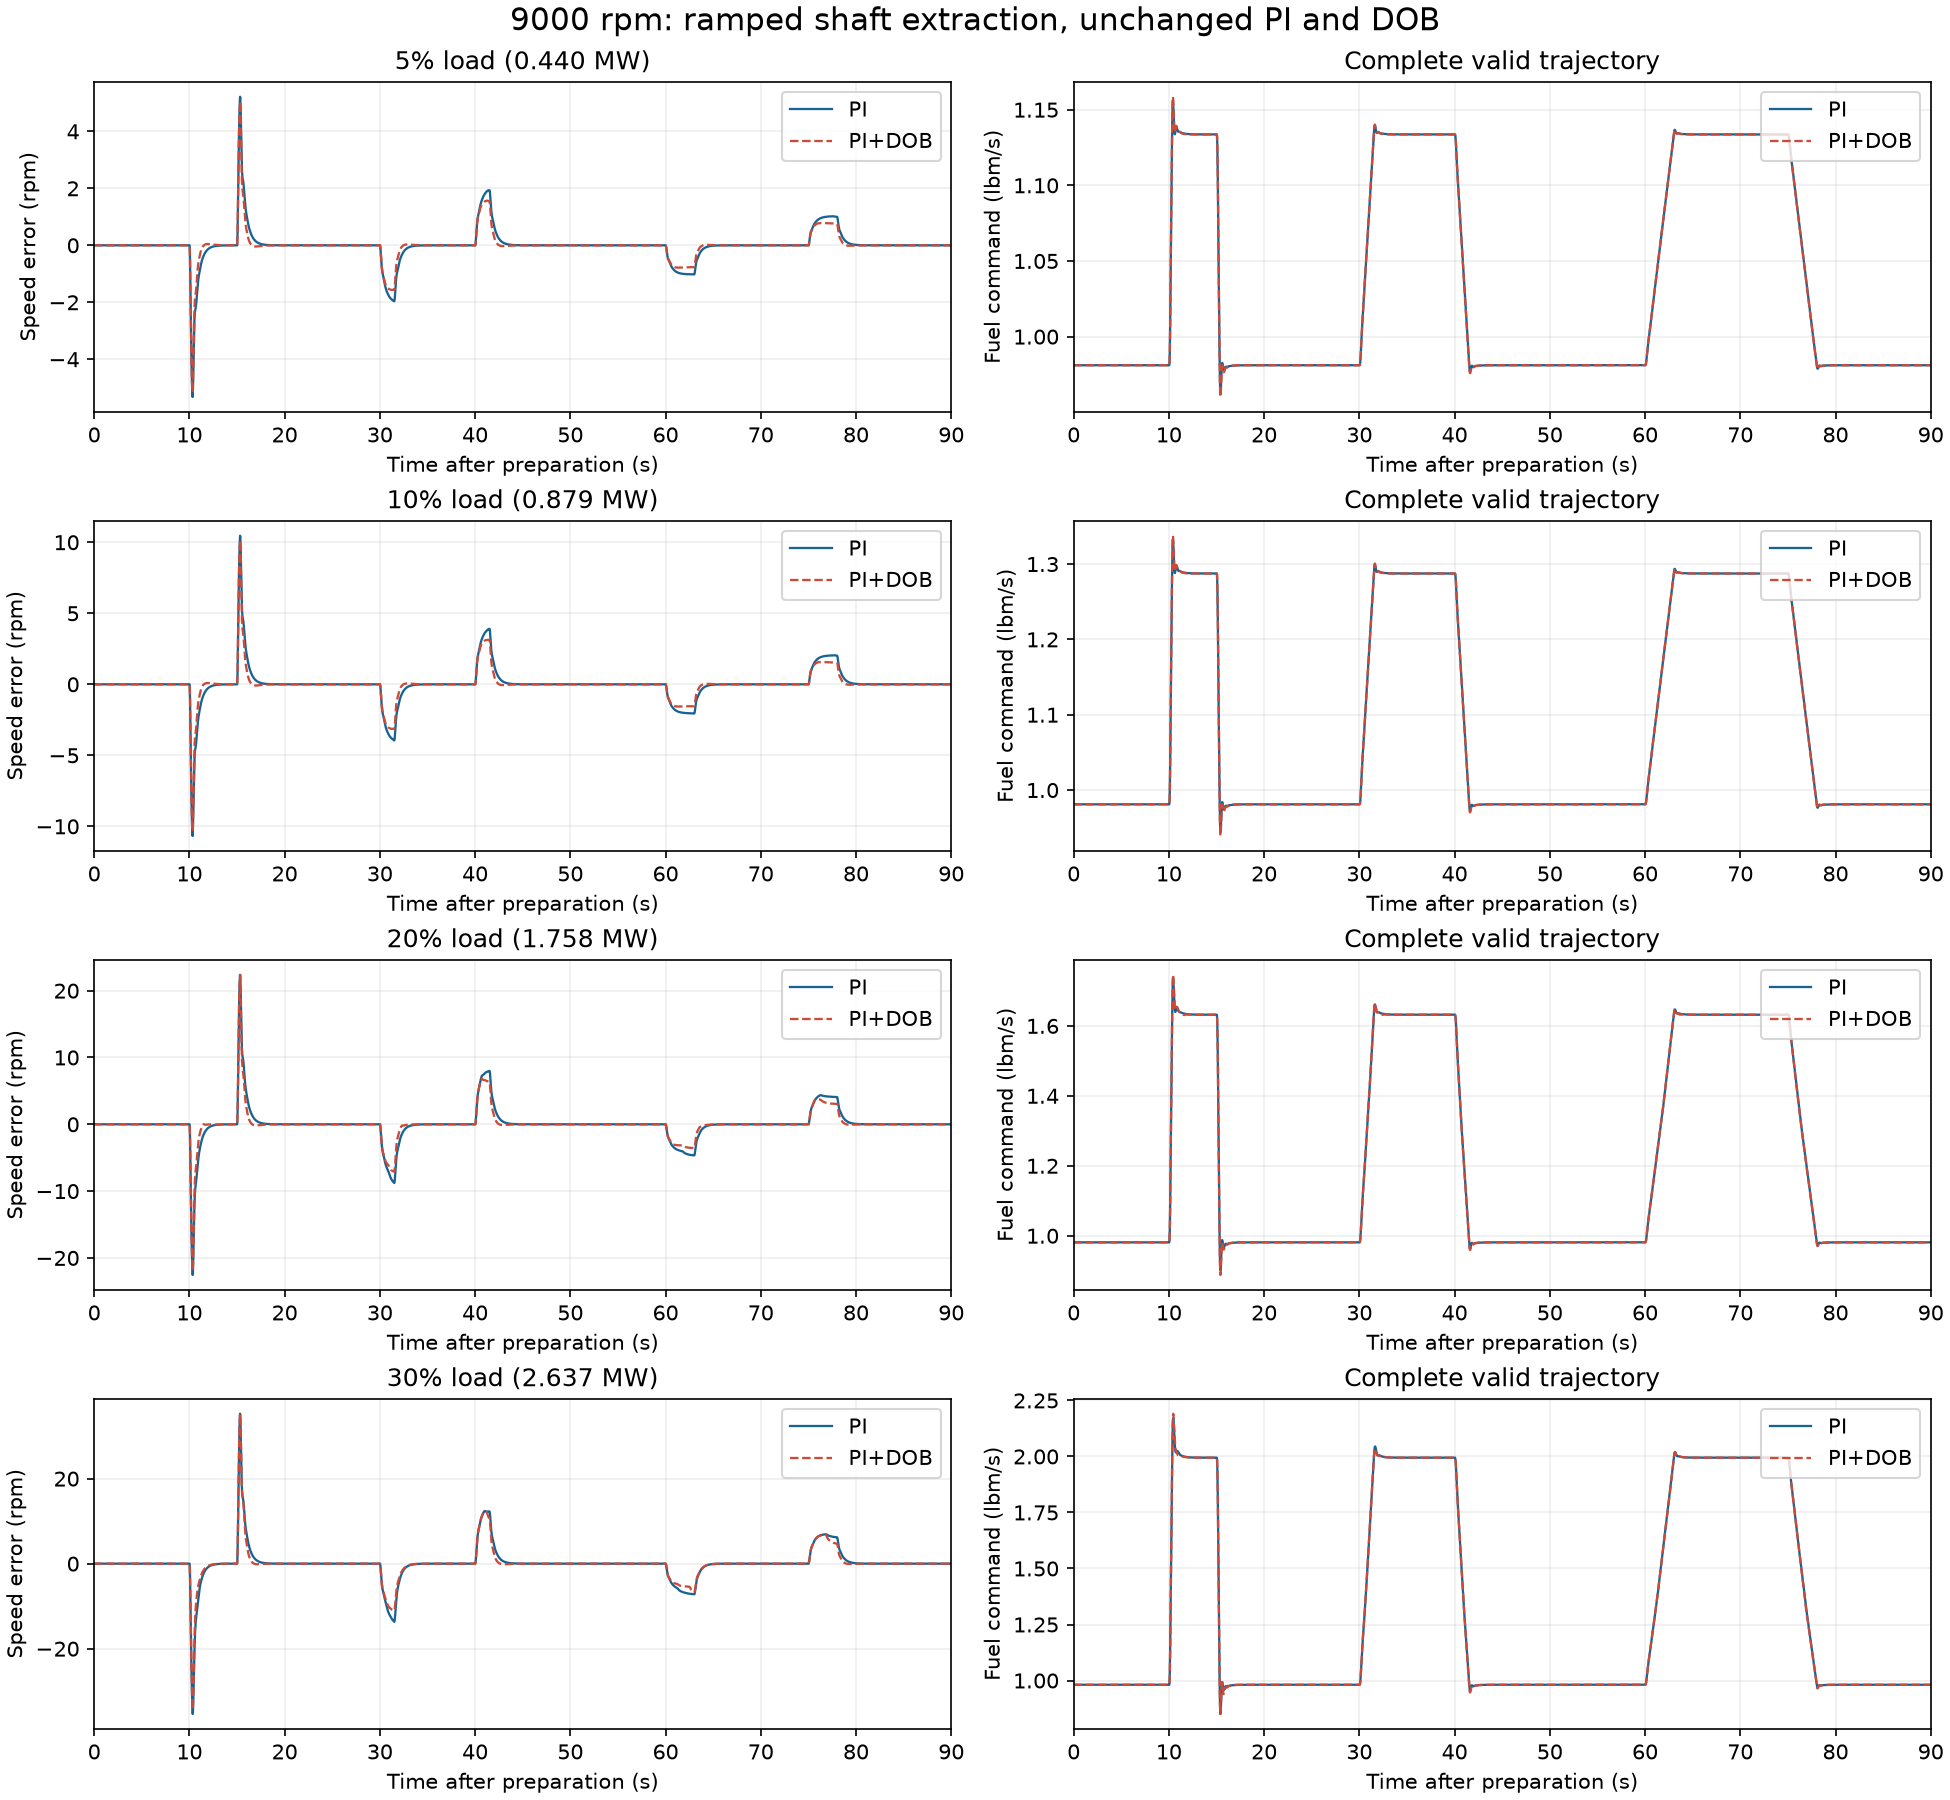
\includegraphics[width=.95\linewidth,height=.6\textheight,keepaspectratio]{early_PTO_9000rpm_ramp_comparison_overview.png}\caption{Overview. Archived study figure.}\end{figure}

\subsection{Time response at each ramp}

Recovery is the first sample after the last excursion outside $\pm$1 rpm, confirmed by at least 0.5 s within the band through the next ramp start. After-ramp recovery is max(0, recovery from start - ramp duration). A zero means recovery occurred by ramp completion. Metrics are withheld for an event if any earlier plant solve was invalid. A dash can also mean no confirmed settling.

{\scriptsize\setlength{\tabcolsep}{1.5mm}\begin{longtable}{>{\raggedright\arraybackslash}p{19.86mm}>{\raggedright\arraybackslash}p{19.86mm}>{\raggedright\arraybackslash}p{19.86mm}>{\raggedright\arraybackslash}p{19.86mm}>{\raggedright\arraybackslash}p{19.86mm}>{\raggedright\arraybackslash}p{19.86mm}>{\raggedright\arraybackslash}p{19.86mm}}\caption{The 9000-rpm ramped-load envelope: Time response at each ramp. Archived values.}\\\toprule
Load & Ramp s & Edge & Controller & Peak error rpm & Recovery from start s & After ramp s\\\midrule
\endfirsthead
Load & Ramp s & Edge & Controller & Peak error rpm & Recovery from start s & After ramp s\\\midrule
\endhead
5\% & 0.30 & application & PI & 5.325 & 1.035 & 0.735\\
5\% & 0.30 & removal & PI & 5.215 & 1.050 & 0.750\\
5\% & 1.50 & application & PI & 1.965 & 1.785 & 0.285\\
5\% & 1.50 & removal & PI & 1.932 & 1.785 & 0.285\\
5\% & 3.00 & application & PI & 1.020 & 3.045 & 0.045\\
5\% & 3.00 & removal & PI & 1.020 & 2.985 & 0.000\\
5\% & 0.30 & application & PI+DOB & 5.162 & 0.825 & 0.525\\
5\% & 0.30 & removal & PI+DOB & 5.055 & 0.825 & 0.525\\
5\% & 1.50 & application & PI+DOB & 1.565 & 1.665 & 0.165\\
5\% & 1.50 & removal & PI+DOB & 1.567 & 1.650 & 0.150\\
5\% & 3.00 & application & PI+DOB & 0.784 & 0.000 & 0.000\\
5\% & 3.00 & removal & PI+DOB & 0.782 & 0.000 & 0.000\\
10\% & 0.30 & application & PI & 10.677 & 1.350 & 1.050\\
10\% & 0.30 & removal & PI & 10.457 & 1.380 & 1.080\\
10\% & 1.50 & application & PI & 3.950 & 2.130 & 0.630\\
10\% & 1.50 & removal & PI & 3.901 & 2.145 & 0.645\\
10\% & 3.00 & application & PI & 2.054 & 3.315 & 0.315\\
10\% & 3.00 & removal & PI & 2.042 & 3.315 & 0.315\\
10\% & 0.30 & application & PI+DOB & 10.351 & 1.005 & 0.705\\
10\% & 0.30 & removal & PI+DOB & 10.140 & 1.035 & 0.735\\
10\% & 1.50 & application & PI+DOB & 3.145 & 1.845 & 0.345\\
10\% & 1.50 & removal & PI+DOB & 3.134 & 1.860 & 0.360\\
10\% & 3.00 & application & PI+DOB & 1.565 & 3.165 & 0.165\\
10\% & 3.00 & removal & PI+DOB & 1.566 & 3.150 & 0.150\\
20\% & 0.30 & application & PI & 22.553 & 1.695 & 1.395\\
20\% & 0.30 & removal & PI & 22.380 & 1.740 & 1.440\\
20\% & 1.50 & application & PI & 8.786 & 2.490 & 0.990\\
20\% & 1.50 & removal & PI & 7.988 & 2.490 & 0.990\\
20\% & 3.00 & application & PI & 4.649 & 3.705 & 0.705\\
20\% & 3.00 & removal & PI & 4.363 & 3.660 & 0.660\\
20\% & 0.30 & application & PI+DOB & 21.914 & 1.170 & 0.870\\
20\% & 0.30 & removal & PI+DOB & 22.329 & 1.215 & 0.915\\
20\% & 1.50 & application & PI+DOB & 7.096 & 2.055 & 0.555\\
20\% & 1.50 & removal & PI+DOB & 6.823 & 2.040 & 0.540\\
20\% & 3.00 & application & PI+DOB & 3.536 & 3.360 & 0.360\\
20\% & 3.00 & removal & PI+DOB & 3.771 & 3.345 & 0.345\\
30\% & 0.30 & application & PI & 35.359 & 1.875 & 1.575\\
30\% & 0.30 & removal & PI & 35.257 & 1.950 & 1.650\\
30\% & 1.50 & application & PI & 13.677 & 2.685 & 1.185\\
30\% & 1.50 & removal & PI & 12.372 & 2.700 & 1.200\\
30\% & 3.00 & application & PI & 7.239 & 3.900 & 0.900\\
30\% & 3.00 & removal & PI & 6.909 & 3.870 & 0.870\\
30\% & 0.30 & application & PI+DOB & 34.333 & 1.680 & 1.380\\
30\% & 0.30 & removal & PI+DOB & 35.258 & 1.410 & 1.110\\
30\% & 1.50 & application & PI+DOB & 11.032 & 2.580 & 1.080\\
30\% & 1.50 & removal & PI+DOB & 12.372 & 2.190 & 0.690\\
30\% & 3.00 & application & PI+DOB & 6.730 & 3.870 & 0.870\\
30\% & 3.00 & removal & PI+DOB & 6.901 & 3.480 & 0.480\\
\bottomrule\end{longtable}}

\subsection{Ramp rates}

{\scriptsize\setlength{\tabcolsep}{1.5mm}\begin{longtable}{>{\raggedright\arraybackslash}p{37.00mm}>{\raggedright\arraybackslash}p{37.00mm}>{\raggedright\arraybackslash}p{37.00mm}>{\raggedright\arraybackslash}p{37.00mm}}\caption{The 9000-rpm ramped-load envelope: Ramp rates. Archived values.}\\\toprule
Load & 0.30 s ramp (MW/s) & 1.50 s ramp (MW/s) & 3.00 s ramp (MW/s)\\\midrule
\endfirsthead
Load & 0.30 s ramp (MW/s) & 1.50 s ramp (MW/s) & 3.00 s ramp (MW/s)\\\midrule
\endhead
5\% & 1.465 & 0.293 & 0.147\\
10\% & 2.930 & 0.586 & 0.293\\
20\% & 5.861 & 1.172 & 0.586\\
30\% & 8.791 & 1.758 & 0.879\\
\bottomrule\end{longtable}}

These magnitudes apply to both rising and falling ramps. The source is sampled and held at 15 ms.

\subsection{Interpretation}

\par\noindent\textbullet\ \textbf{5\%:} observer RMSE changes by -13.03\% relative to PI. Peak absolute error changes from 5.325 to 5.162 rpm. Minimum compressor margin is 29.404\% / 29.347\% (PI / DOB). DOB compensation clips for 0.00\% of evaluation samples.
\par\noindent\textbullet\ \textbf{10\%:} observer RMSE changes by -13.02\% relative to PI. Peak absolute error changes from 10.677 to 10.351 rpm. Minimum compressor margin is 24.429\% / 24.322\% (PI / DOB). DOB compensation clips for 0.00\% of evaluation samples.
\par\noindent\textbullet\ \textbf{20\%:} observer RMSE changes by -11.92\% relative to PI. Peak absolute error changes from 22.553 to 22.329 rpm. Minimum compressor margin is 14.445\% / 14.238\% (PI / DOB). DOB compensation clips for 26.98\% of evaluation samples.
\par\noindent\textbullet\ \textbf{30\%:} observer RMSE changes by -7.77\% relative to PI. Peak absolute error changes from 35.359 to 35.258 rpm. Minimum compressor margin is 5.526\% / 5.231\% (PI / DOB). DOB compensation clips for 31.98\% of evaluation samples.

At 30\% load, increasing the application ramp from 0.30 to 3.00 s reduces PI peak error from 35.359 to 7.239 rpm and DOB peak error from 34.333 to 6.730 rpm. However, on the 3.00 s application ramp the observer improves recovery after completion by only 0.030 s (0.900 to 0.870 s). On the 0.30 s removal ramp, the peak is effectively unchanged (35.257 versus 35.258 rpm), while after-ramp recovery improves from 1.650 to 1.110 s. This supports a recovery benefit, not uniform peak suppression. At 5\% with a 3.00 s ramp, DOB error stays within $\pm$1 rpm throughout both events.

All eight trajectories pass the numerical checks, with no fuel saturation. At 30\%, DOB peak fuel is 2.191 lbm/s and minimum reported compressor margin is 5.231\%. The lower margin and frequent compensation clipping motivate constraint-aware tuning before extending the load envelope. Compared with the earlier 9500 rpm step tests, both the operating point, absolute load and disturbance shape have changed: 30\% is now 2.637 MW rather than 4.286 MW. The valid result cannot be attributed solely to observer performance or solely to ramp shaping.

The DOB is bounded equivalent-input compensation around the existing PI loop. It estimates the combined effect of external load and nominal-model mismatch; its estimate is not a calibrated shaft-power measurement. Slower ramps generally give the controller more time to compensate, but the event table is the evidence for this plant: peak rejection, settling and global RMSE need not improve together. The three ramp rates share a trajectory with different preceding histories and hold lengths, so these are representative scenarios rather than independent rate-identification experiments.

The fixed model was identified from fuel-to-acceleration data and corrected for zero equilibrium acceleration before observer synthesis. Its inverse and low-pass filtering introduce a bandwidth tradeoff: stronger/faster compensation can improve rejection while amplifying sensor noise and model error. Compensation clipping limits authority. PI integral action provides steady regulation; no anti-windup was added for these comparisons.

Next steps are independent runs for each rate with identical settling windows, gain scheduling across operating points, sensor-noise and delay tests, anti-windup and explicit fuel, temperature, and compressor-margin constraints, then fixed-step embedded timing and hardware-in-the-loop assessment. If flow convergence fails, first establish a numerically valid operating envelope; an invalid trajectory is not proof of physical instability or surge.

\subsection{Verification and reproduction}

The two controllers receive identical sampled power profiles, verified against the ramp formula. Each run has 10001 samples through 150 s. The mechanical torque balance is reconstructed from logged turbine, compressor and external powers and checked against shaft acceleration. Validity requires finite signals, positive fuel and compressor margin, flow residual $\le$1e-9 and fewer than 200 solver iterations. All plots show only the prefix before the first invalid solve. Full raw trajectories are retained for diagnosis.

Run \path|run_tmats_pto_9000_ramp_batch| in MATLAB, then \path|summarize_pto_9000_ramps.py| in Python for the report. A single level is \texttt{out=run\_\allowbreak tmats\_\allowbreak pto\_\allowbreak study(0.10,9000,[0.30} \texttt{1.50} \texttt{3.00]);}. Omitting the third argument preserves the earlier step-load study. The existing PTO Simulink model is unchanged.

\subsection{5\% response zooms}

\begin{figure}[H]\centering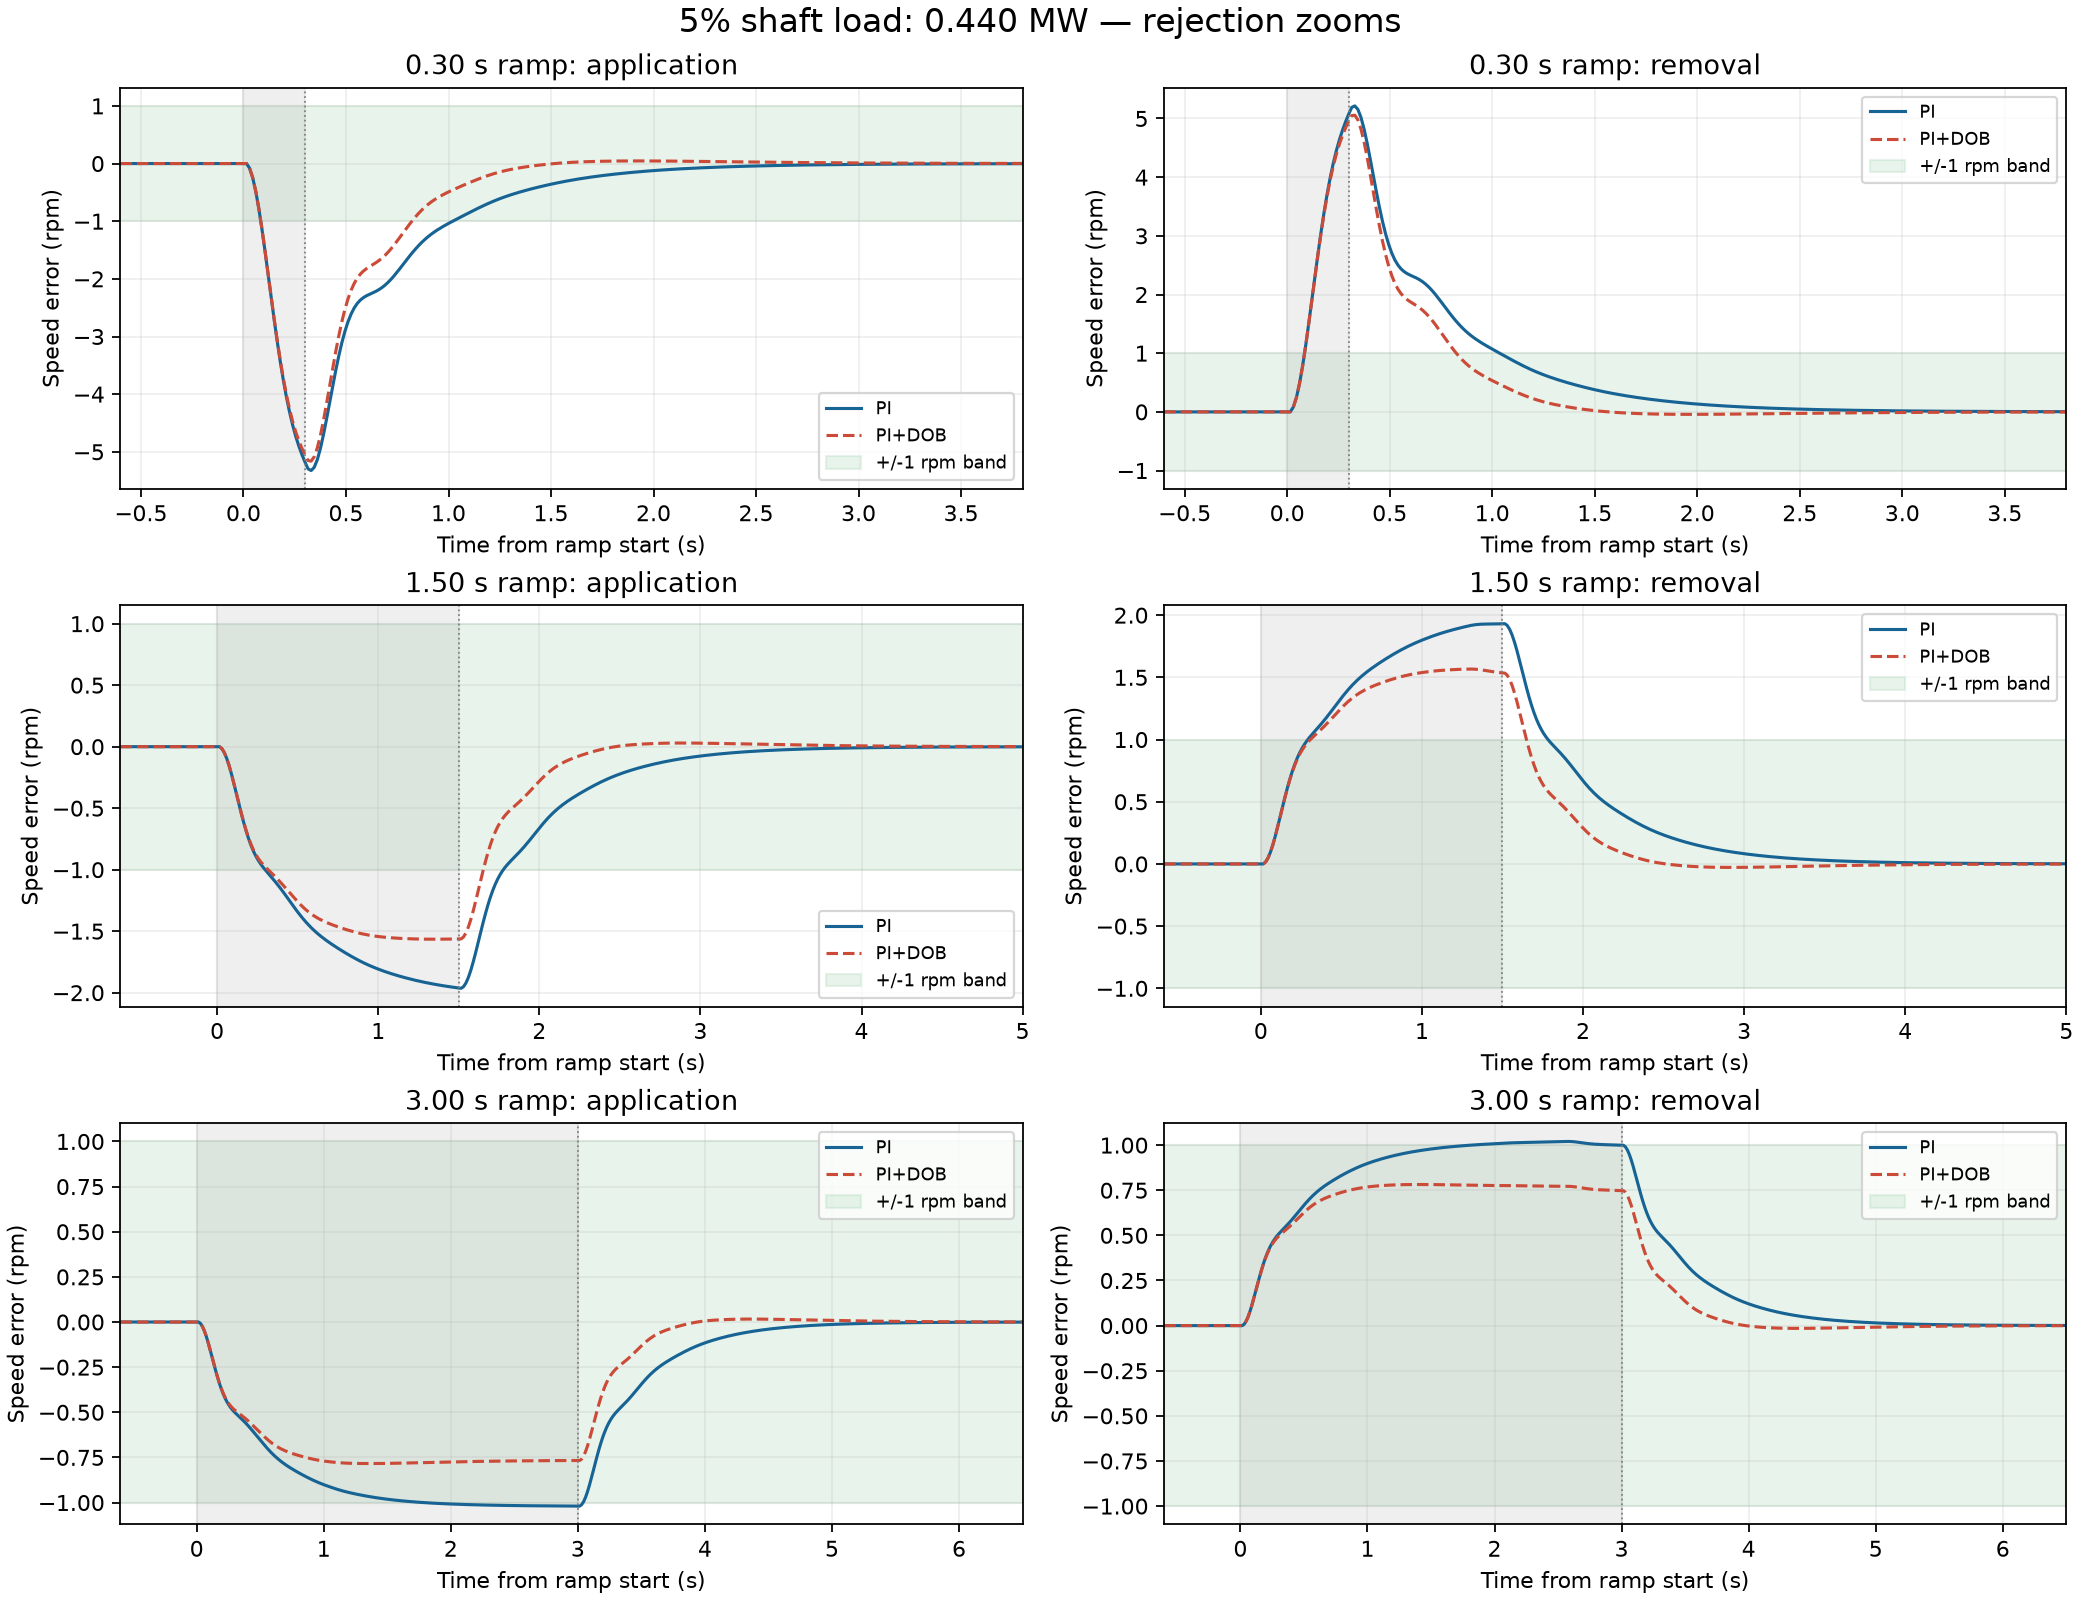
\includegraphics[width=.95\linewidth,height=.6\textheight,keepaspectratio]{early_PTO_9000rpm_ramp_comparison_zoom_05pct.png}\caption{5\% zoom. Archived study figure.}\end{figure}

\subsection{10\% response zooms}

\begin{figure}[H]\centering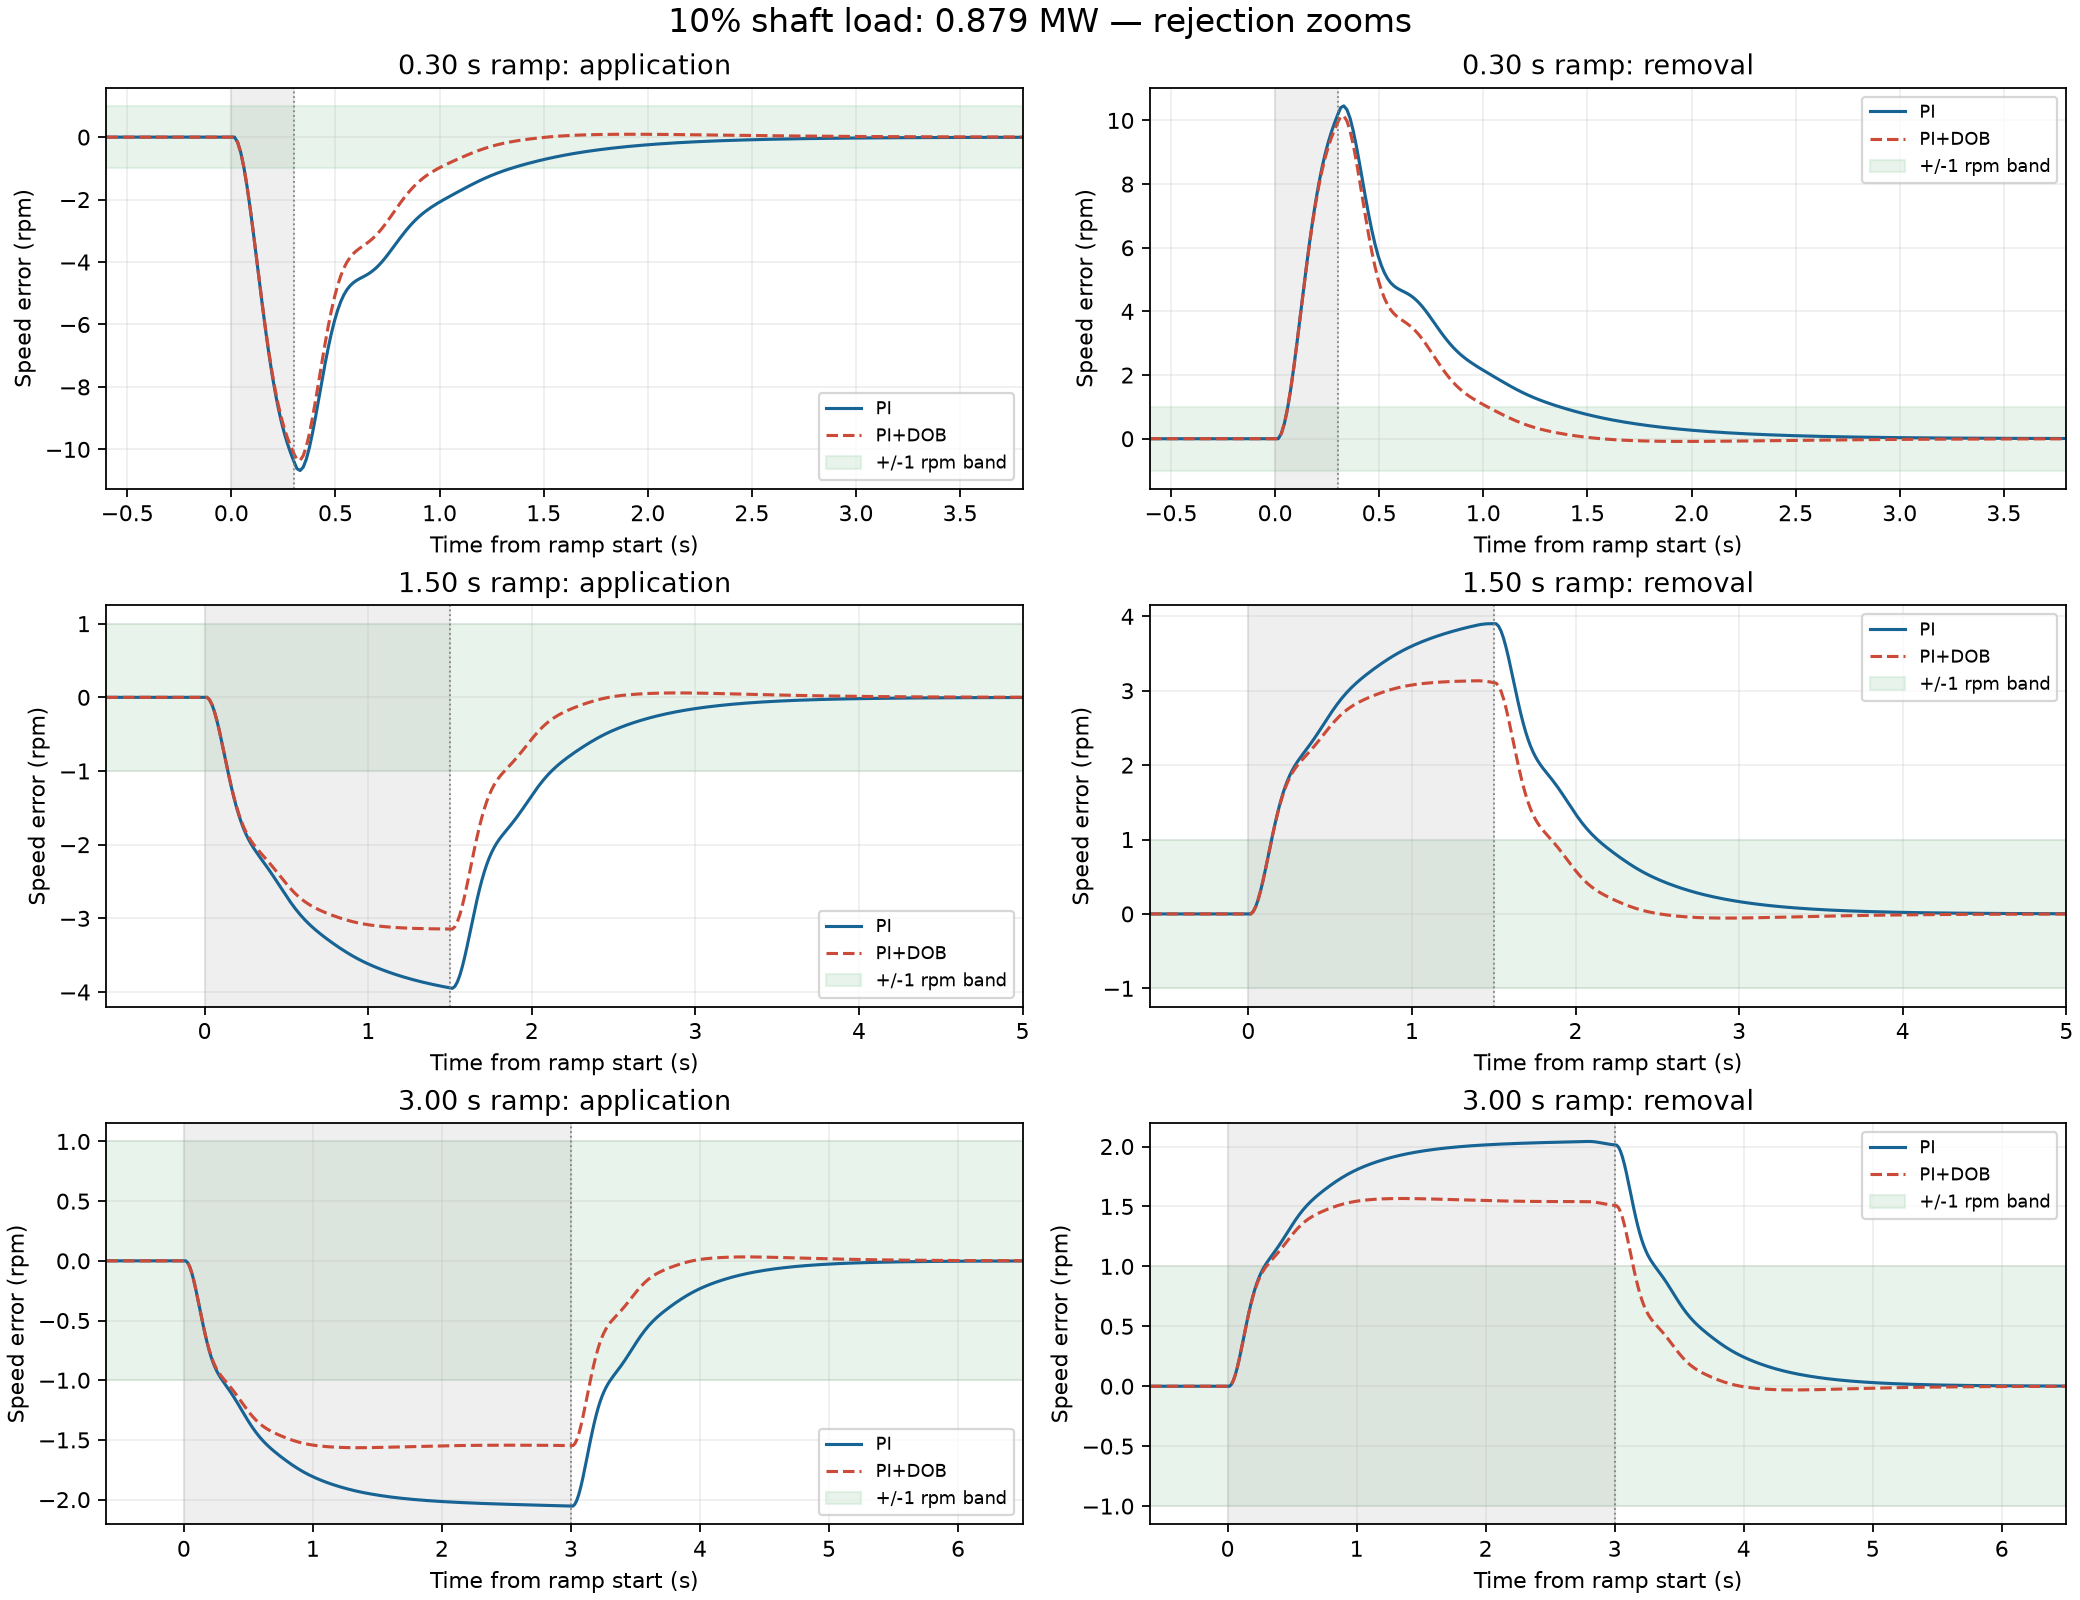
\includegraphics[width=.95\linewidth,height=.6\textheight,keepaspectratio]{early_PTO_9000rpm_ramp_comparison_zoom_10pct.png}\caption{10\% zoom. Archived study figure.}\end{figure}

\subsection{20\% response zooms}

\begin{figure}[H]\centering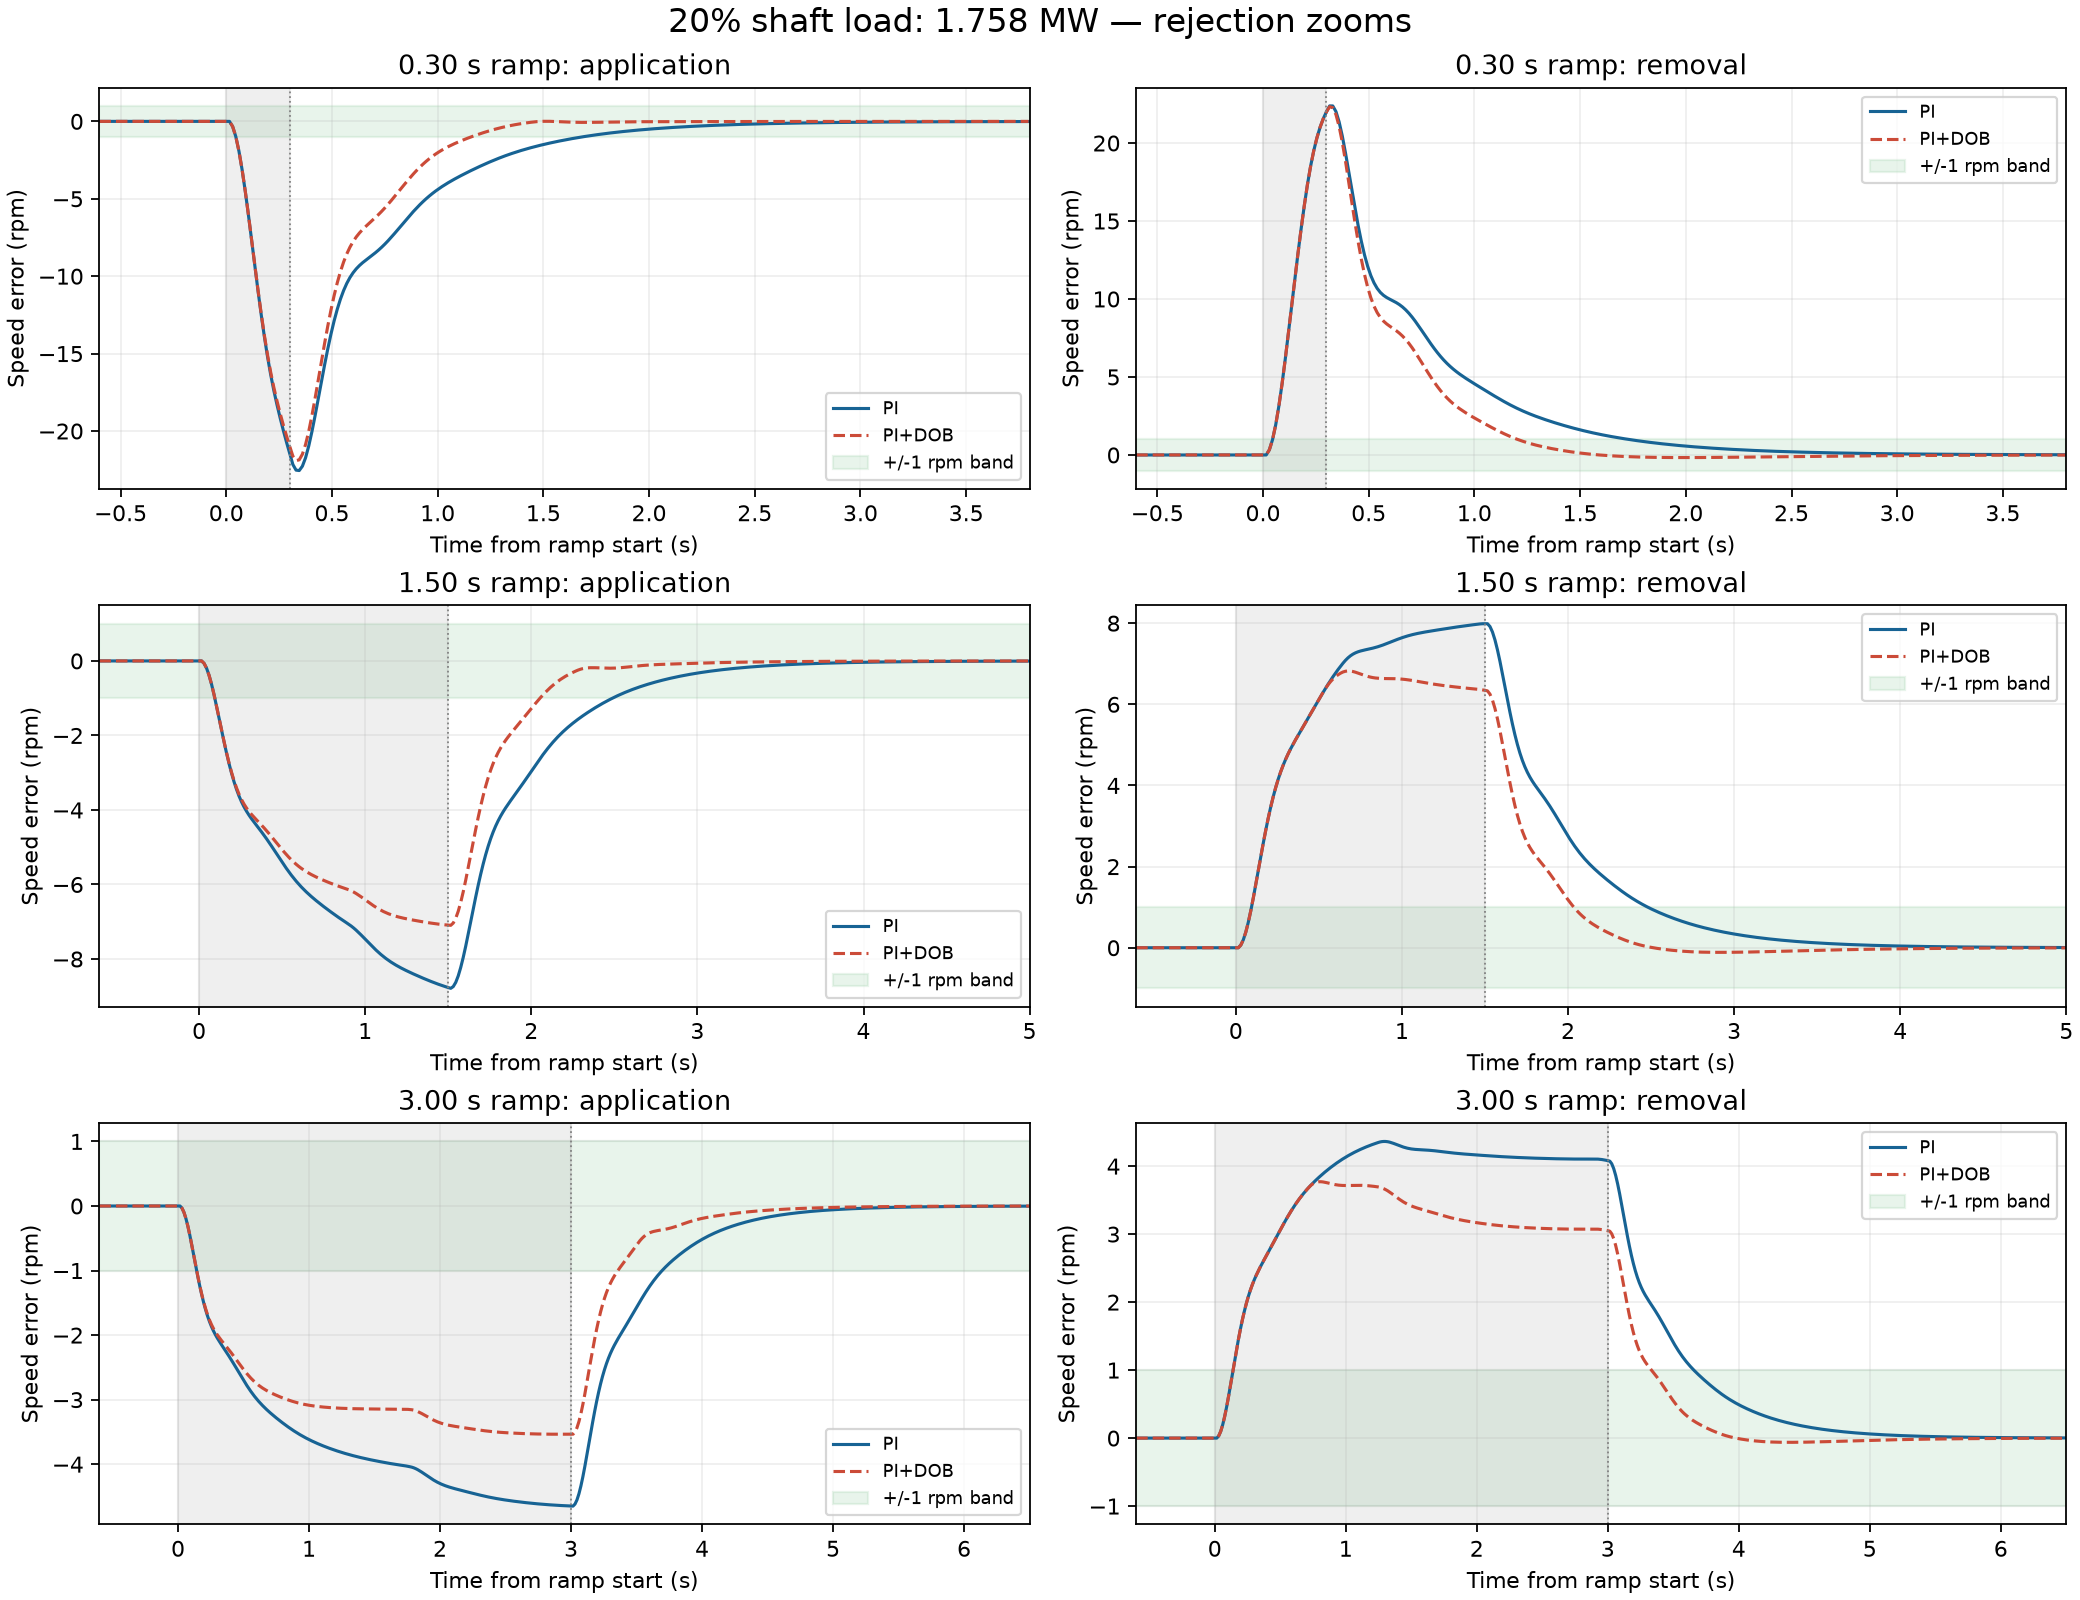
\includegraphics[width=.95\linewidth,height=.6\textheight,keepaspectratio]{early_PTO_9000rpm_ramp_comparison_zoom_20pct.png}\caption{20\% zoom. Archived study figure.}\end{figure}

\subsection{30\% response zooms}

\begin{figure}[H]\centering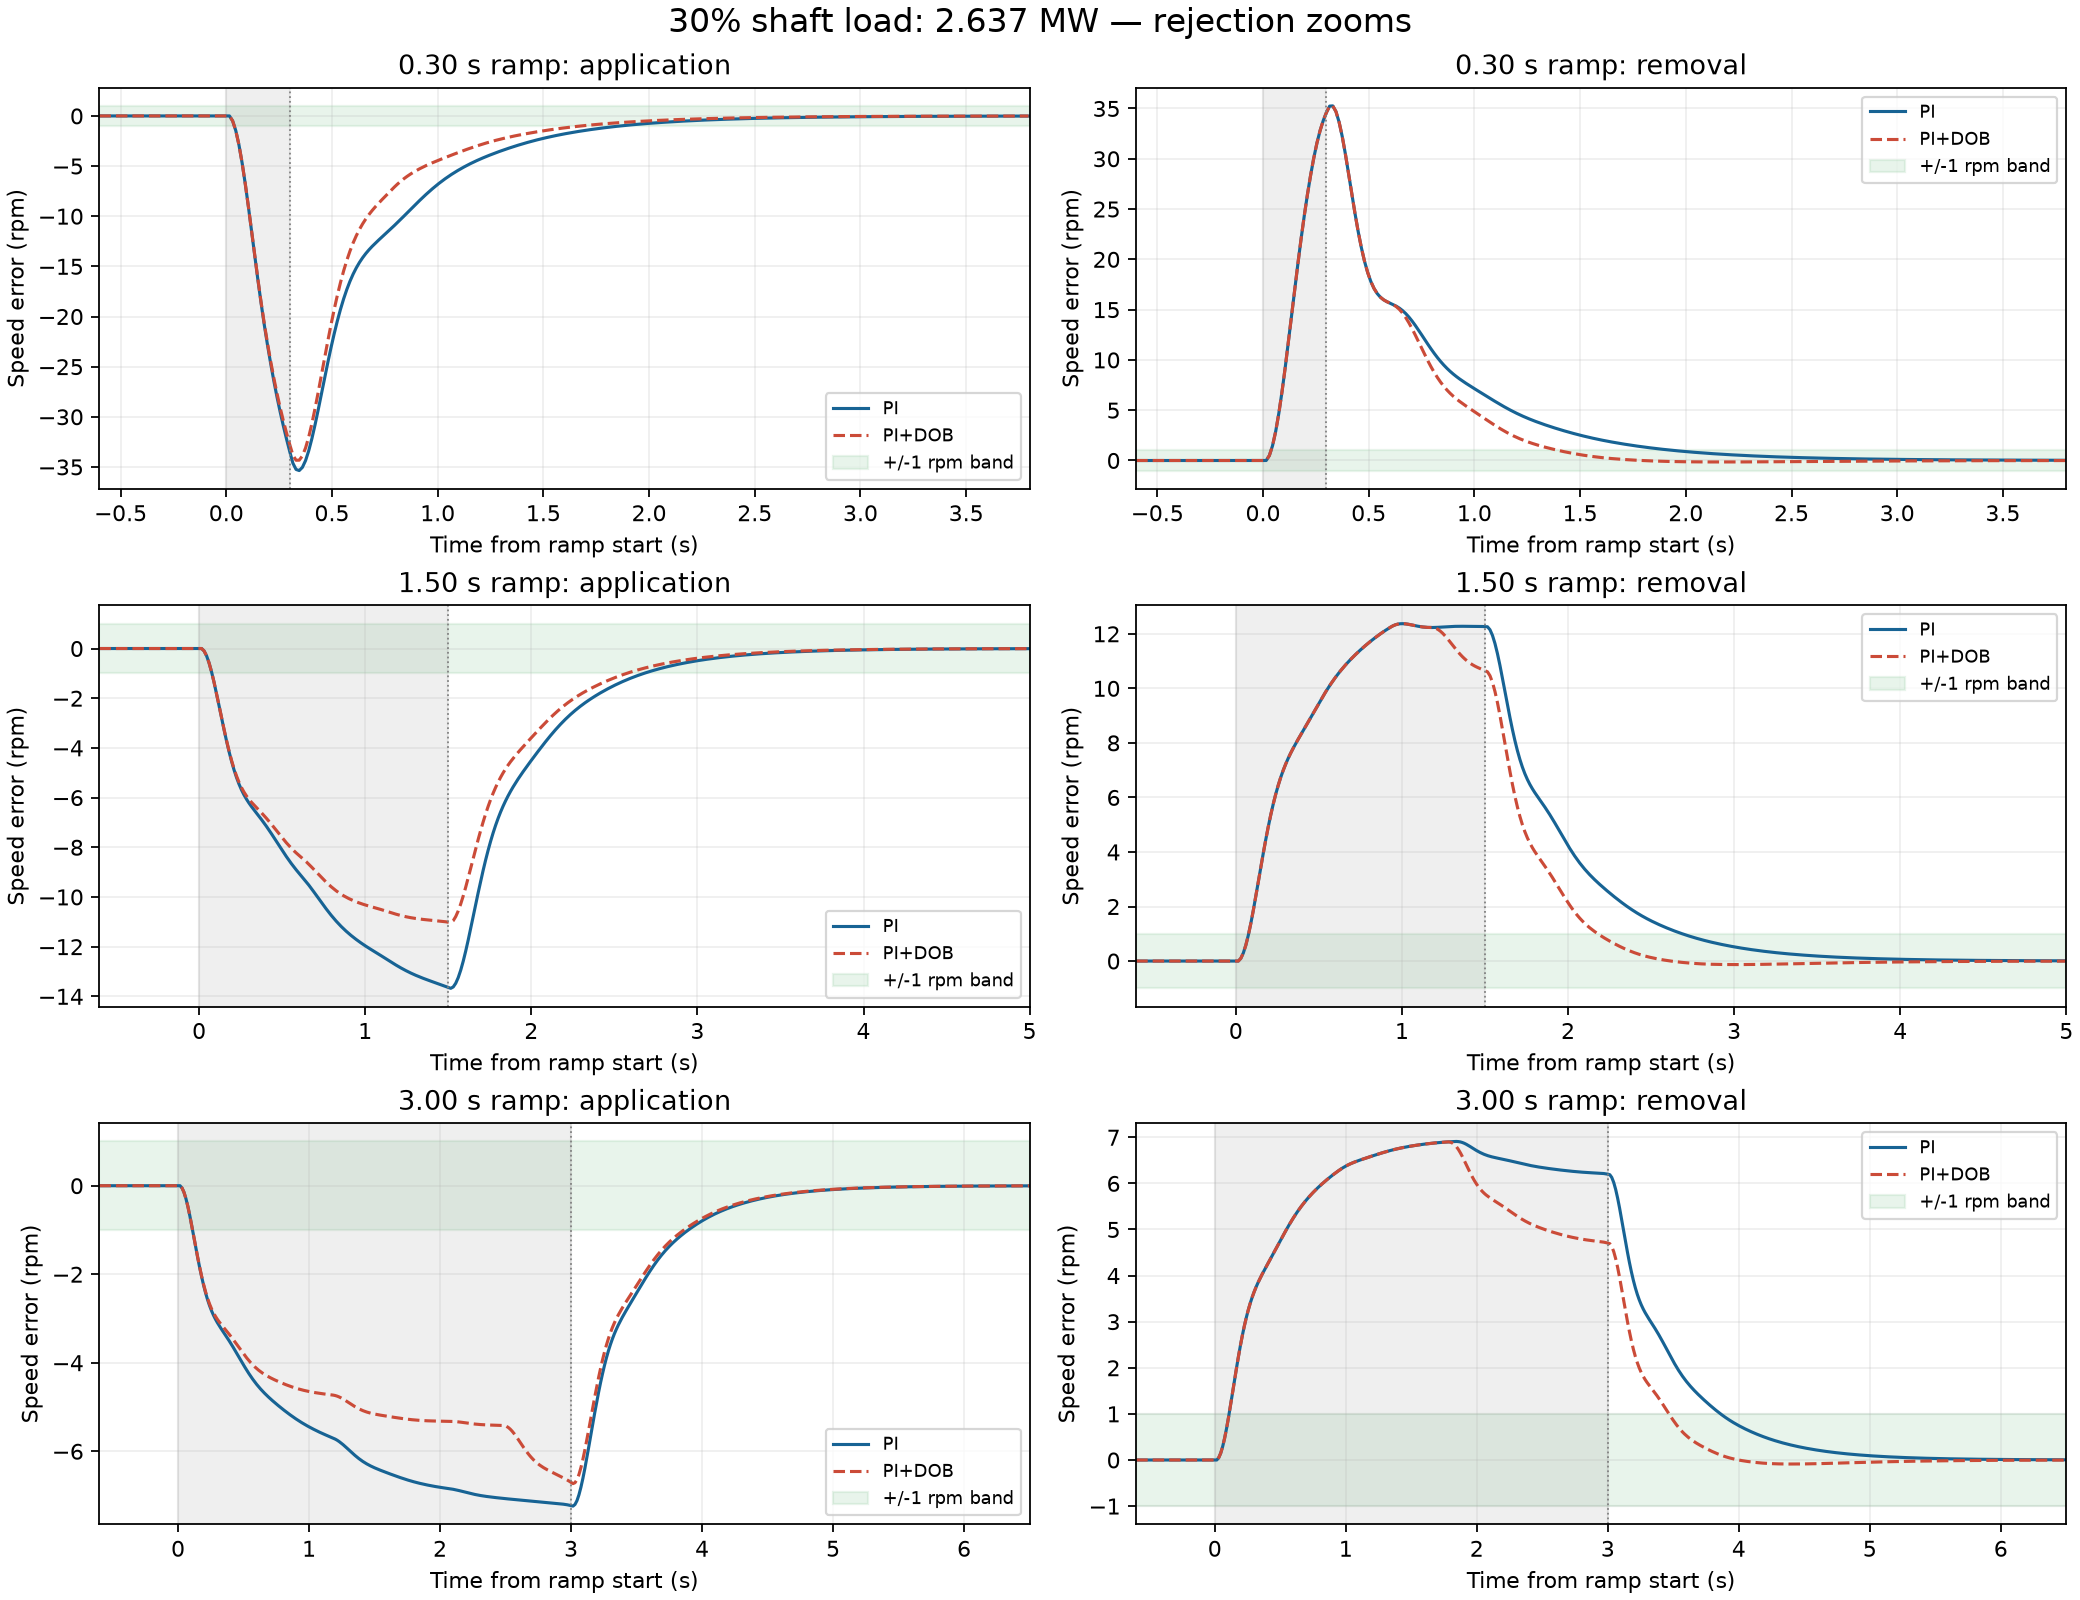
\includegraphics[width=.95\linewidth,height=.6\textheight,keepaspectratio]{early_PTO_9000rpm_ramp_comparison_zoom_30pct.png}\caption{30\% zoom. Archived study figure.}\end{figure}



\section{LESO, UDE, and GPIO implementation and first comparison}
\textit{Evidence basis: }\path|results/literature_observers_9000rpm_10pct_20260912_211600_355/REPORT.md|. The following detailed account is adapted from the archived study; references to simulation and verification describe historical work.\par

Load is \textbf{0.879124 MW} (10\% of 11789.245211 hp gross turbine power). The previous 0.30, 1.50 and 3.00 s ramp/hold/ramp scenario is repeated with five controllers. PI gains, 0.25 compensation gain, $\pm$0.15 lbm/s correction bound, fuel limits and preparation are unchanged. The observer pole-frequency parameter is 0.5 Hz for every method; actual estimator bandwidths differ. No test-based tuning is performed.

The three candidates are LESO (two states), UDE (one state), and ramp GPIO (three states). See the accompanying formulation for equations, primary literature, implementation details and comparison limitations.

\subsection{Measured comparison}

{\scriptsize\setlength{\tabcolsep}{1.5mm}\begin{longtable}{>{\raggedright\arraybackslash}p{19.86mm}>{\raggedright\arraybackslash}p{19.86mm}>{\raggedright\arraybackslash}p{19.86mm}>{\raggedright\arraybackslash}p{19.86mm}>{\raggedright\arraybackslash}p{19.86mm}>{\raggedright\arraybackslash}p{19.86mm}>{\raggedright\arraybackslash}p{19.86mm}}\caption{LESO, UDE, and GPIO implementation and first comparison: Measured comparison. Archived values.}\\\toprule
Method & Valid & RMSE rpm & Reduction vs PI & Peak error rpm & IAE rpm$\cdot$s & Peak fuel lbm/s\\\midrule
\endfirsthead
Method & Valid & RMSE rpm & Reduction vs PI & Peak error rpm & IAE rpm$\cdot$s & Peak fuel lbm/s\\\midrule
\endhead
PI & True & 1.193 & 0.000\% & 10.677 & 36.774 & 1.333\\
DOB & True & 1.038 & 13.021\% & 10.351 & 28.341 & 1.338\\
LESO & True & 1.039 & 12.903\% & 10.349 & 28.694 & 1.338\\
UDE & True & 0.969 & 18.746\% & 9.377 & 27.587 & 1.336\\
GPIO & True & 0.951 & 20.301\% & 9.866 & 27.577 & 1.344\\
\bottomrule\end{longtable}}

\begin{figure}[H]\centering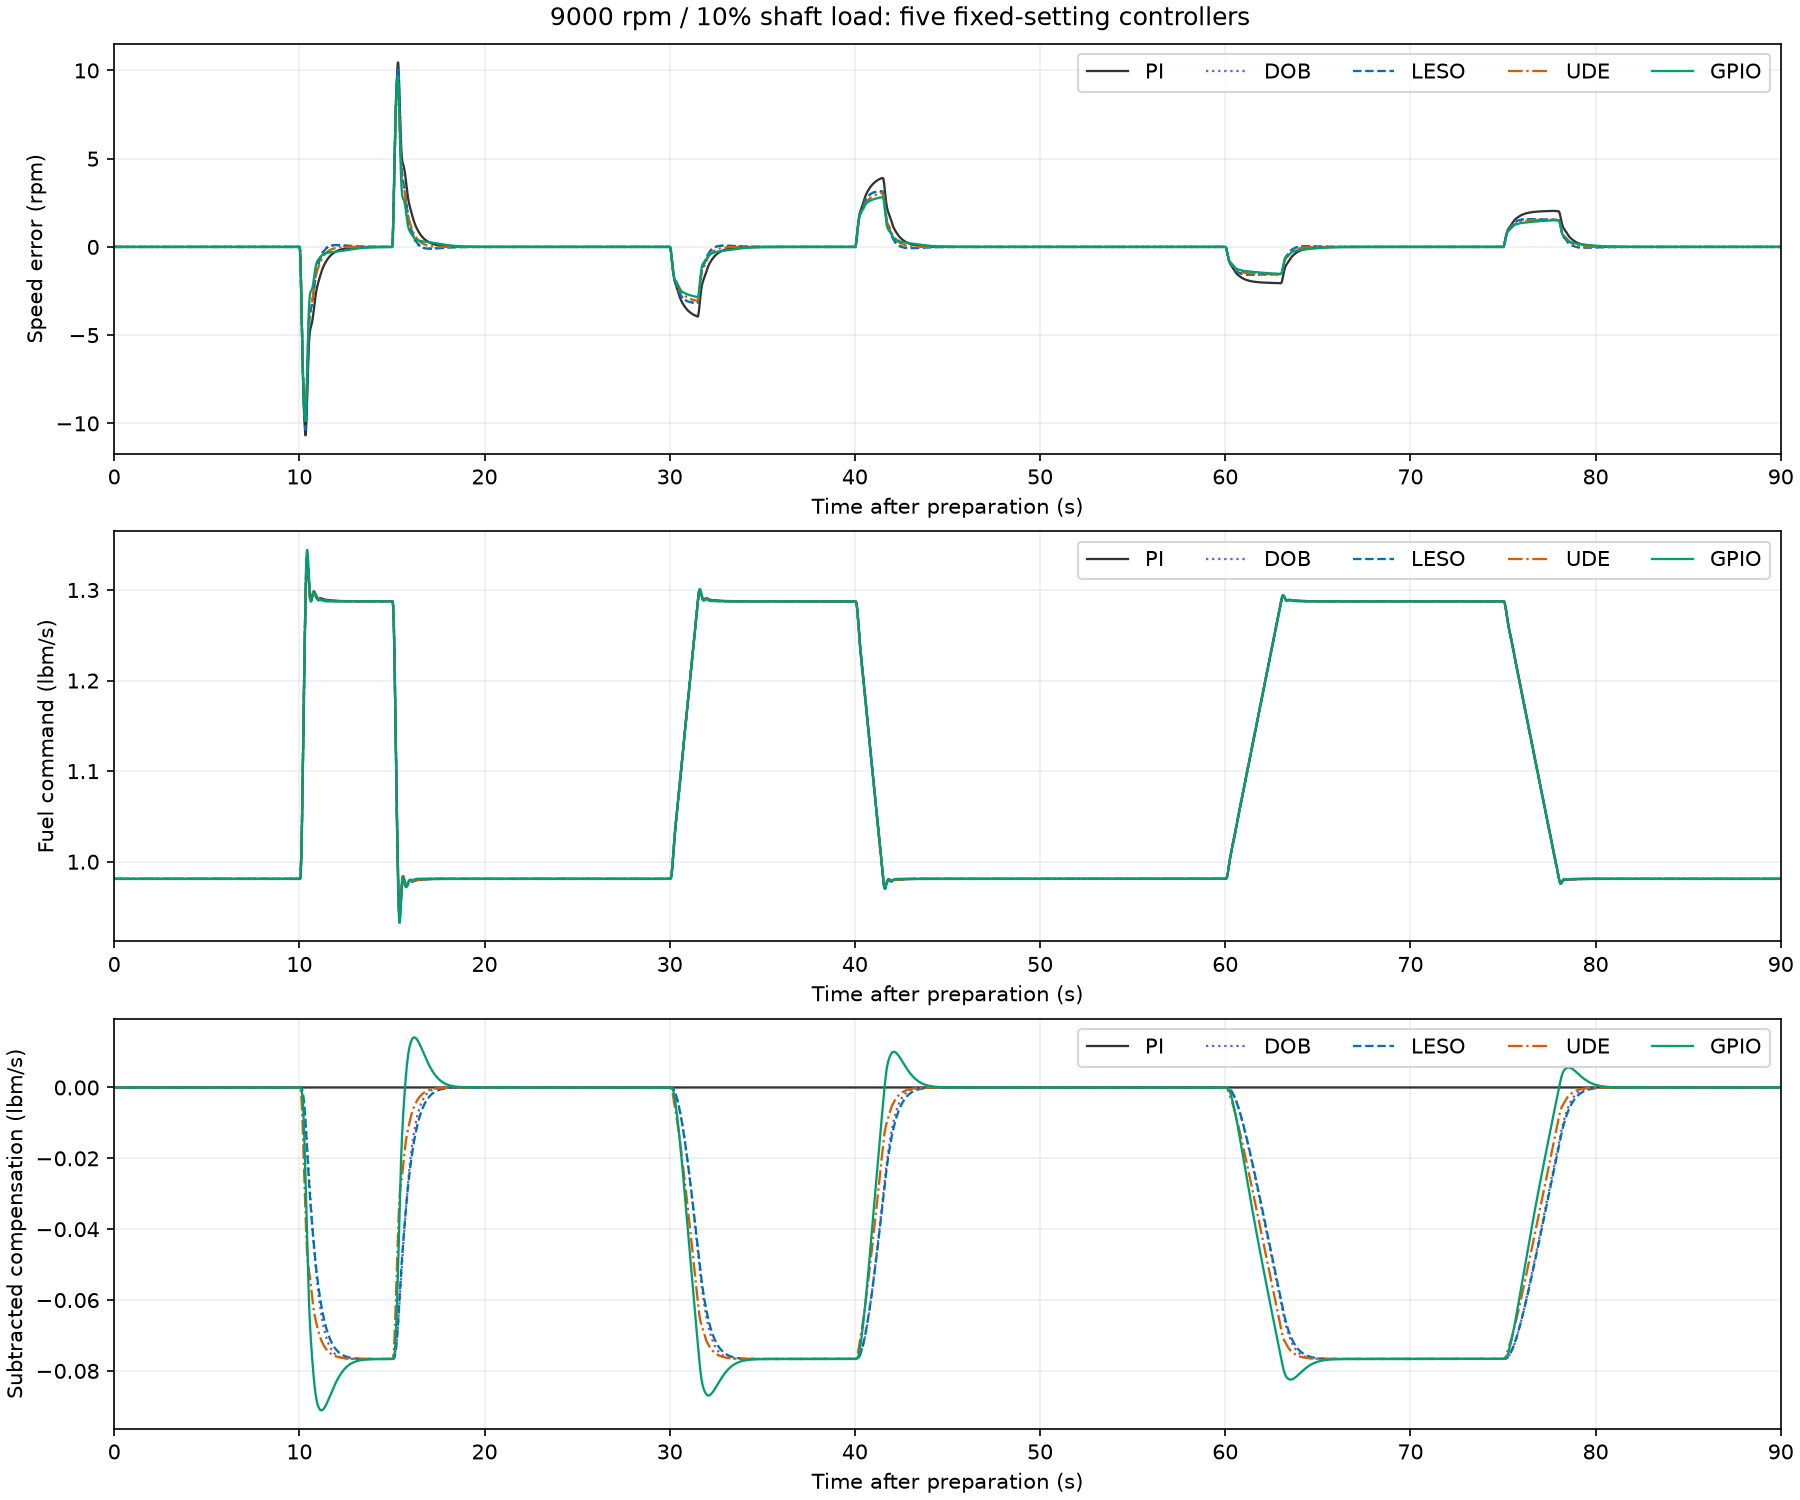
\includegraphics[width=.95\linewidth,height=.6\textheight,keepaspectratio]{early_literature_observers_9000rpm_10pct_20260912_211600_355_overview.png}\caption{Overview. Archived study figure.}\end{figure}

\subsection{Event recovery}

Recovery requires remaining within $\pm$1 rpm to the next ramp, with at least 0.5 s confirmed dwell. After-ramp recovery subtracts the ramp duration, bounded below by zero. Failed propagated trajectories receive no performance claim.

{\scriptsize\setlength{\tabcolsep}{1.5mm}\begin{longtable}{>{\raggedright\arraybackslash}p{23.67mm}>{\raggedright\arraybackslash}p{23.67mm}>{\raggedright\arraybackslash}p{23.67mm}>{\raggedright\arraybackslash}p{23.67mm}>{\raggedright\arraybackslash}p{23.67mm}>{\raggedright\arraybackslash}p{23.67mm}}\caption{LESO, UDE, and GPIO implementation and first comparison: Event recovery. Archived values.}\\\toprule
Ramp s & Edge & Method & Peak rpm & Recovery from start s & After ramp s\\\midrule
\endfirsthead
Ramp s & Edge & Method & Peak rpm & Recovery from start s & After ramp s\\\midrule
\endhead
0.30 & apply & PI & 10.677 & 1.350 & 1.050\\
0.30 & apply & DOB & 10.351 & 1.005 & 0.705\\
0.30 & apply & LESO & 10.349 & 1.020 & 0.720\\
0.30 & apply & UDE & 9.377 & 1.080 & 0.780\\
0.30 & apply & GPIO & 9.866 & 0.915 & 0.615\\
0.30 & remove & PI & 10.457 & 1.380 & 1.080\\
0.30 & remove & DOB & 10.140 & 1.035 & 0.735\\
0.30 & remove & LESO & 10.137 & 1.050 & 0.750\\
0.30 & remove & UDE & 9.205 & 1.095 & 0.795\\
0.30 & remove & GPIO & 9.670 & 0.930 & 0.630\\
1.50 & apply & PI & 3.950 & 2.130 & 0.630\\
1.50 & apply & DOB & 3.145 & 1.845 & 0.345\\
1.50 & apply & LESO & 3.171 & 1.845 & 0.345\\
1.50 & apply & UDE & 3.050 & 1.920 & 0.420\\
1.50 & apply & GPIO & 2.850 & 1.785 & 0.285\\
1.50 & remove & PI & 3.901 & 2.145 & 0.645\\
1.50 & remove & DOB & 3.134 & 1.860 & 0.360\\
1.50 & remove & LESO & 3.158 & 1.875 & 0.375\\
1.50 & remove & UDE & 3.022 & 1.920 & 0.420\\
1.50 & remove & GPIO & 2.817 & 1.800 & 0.300\\
3.00 & apply & PI & 2.054 & 3.315 & 0.315\\
3.00 & apply & DOB & 1.565 & 3.165 & 0.165\\
3.00 & apply & LESO & 1.577 & 3.165 & 0.165\\
3.00 & apply & UDE & 1.545 & 3.165 & 0.165\\
3.00 & apply & GPIO & 1.528 & 3.150 & 0.150\\
3.00 & remove & PI & 2.042 & 3.315 & 0.315\\
3.00 & remove & DOB & 1.566 & 3.150 & 0.150\\
3.00 & remove & LESO & 1.578 & 3.150 & 0.150\\
3.00 & remove & UDE & 1.536 & 3.150 & 0.150\\
3.00 & remove & GPIO & 1.513 & 3.150 & 0.150\\
\bottomrule\end{longtable}}

\begin{figure}[H]\centering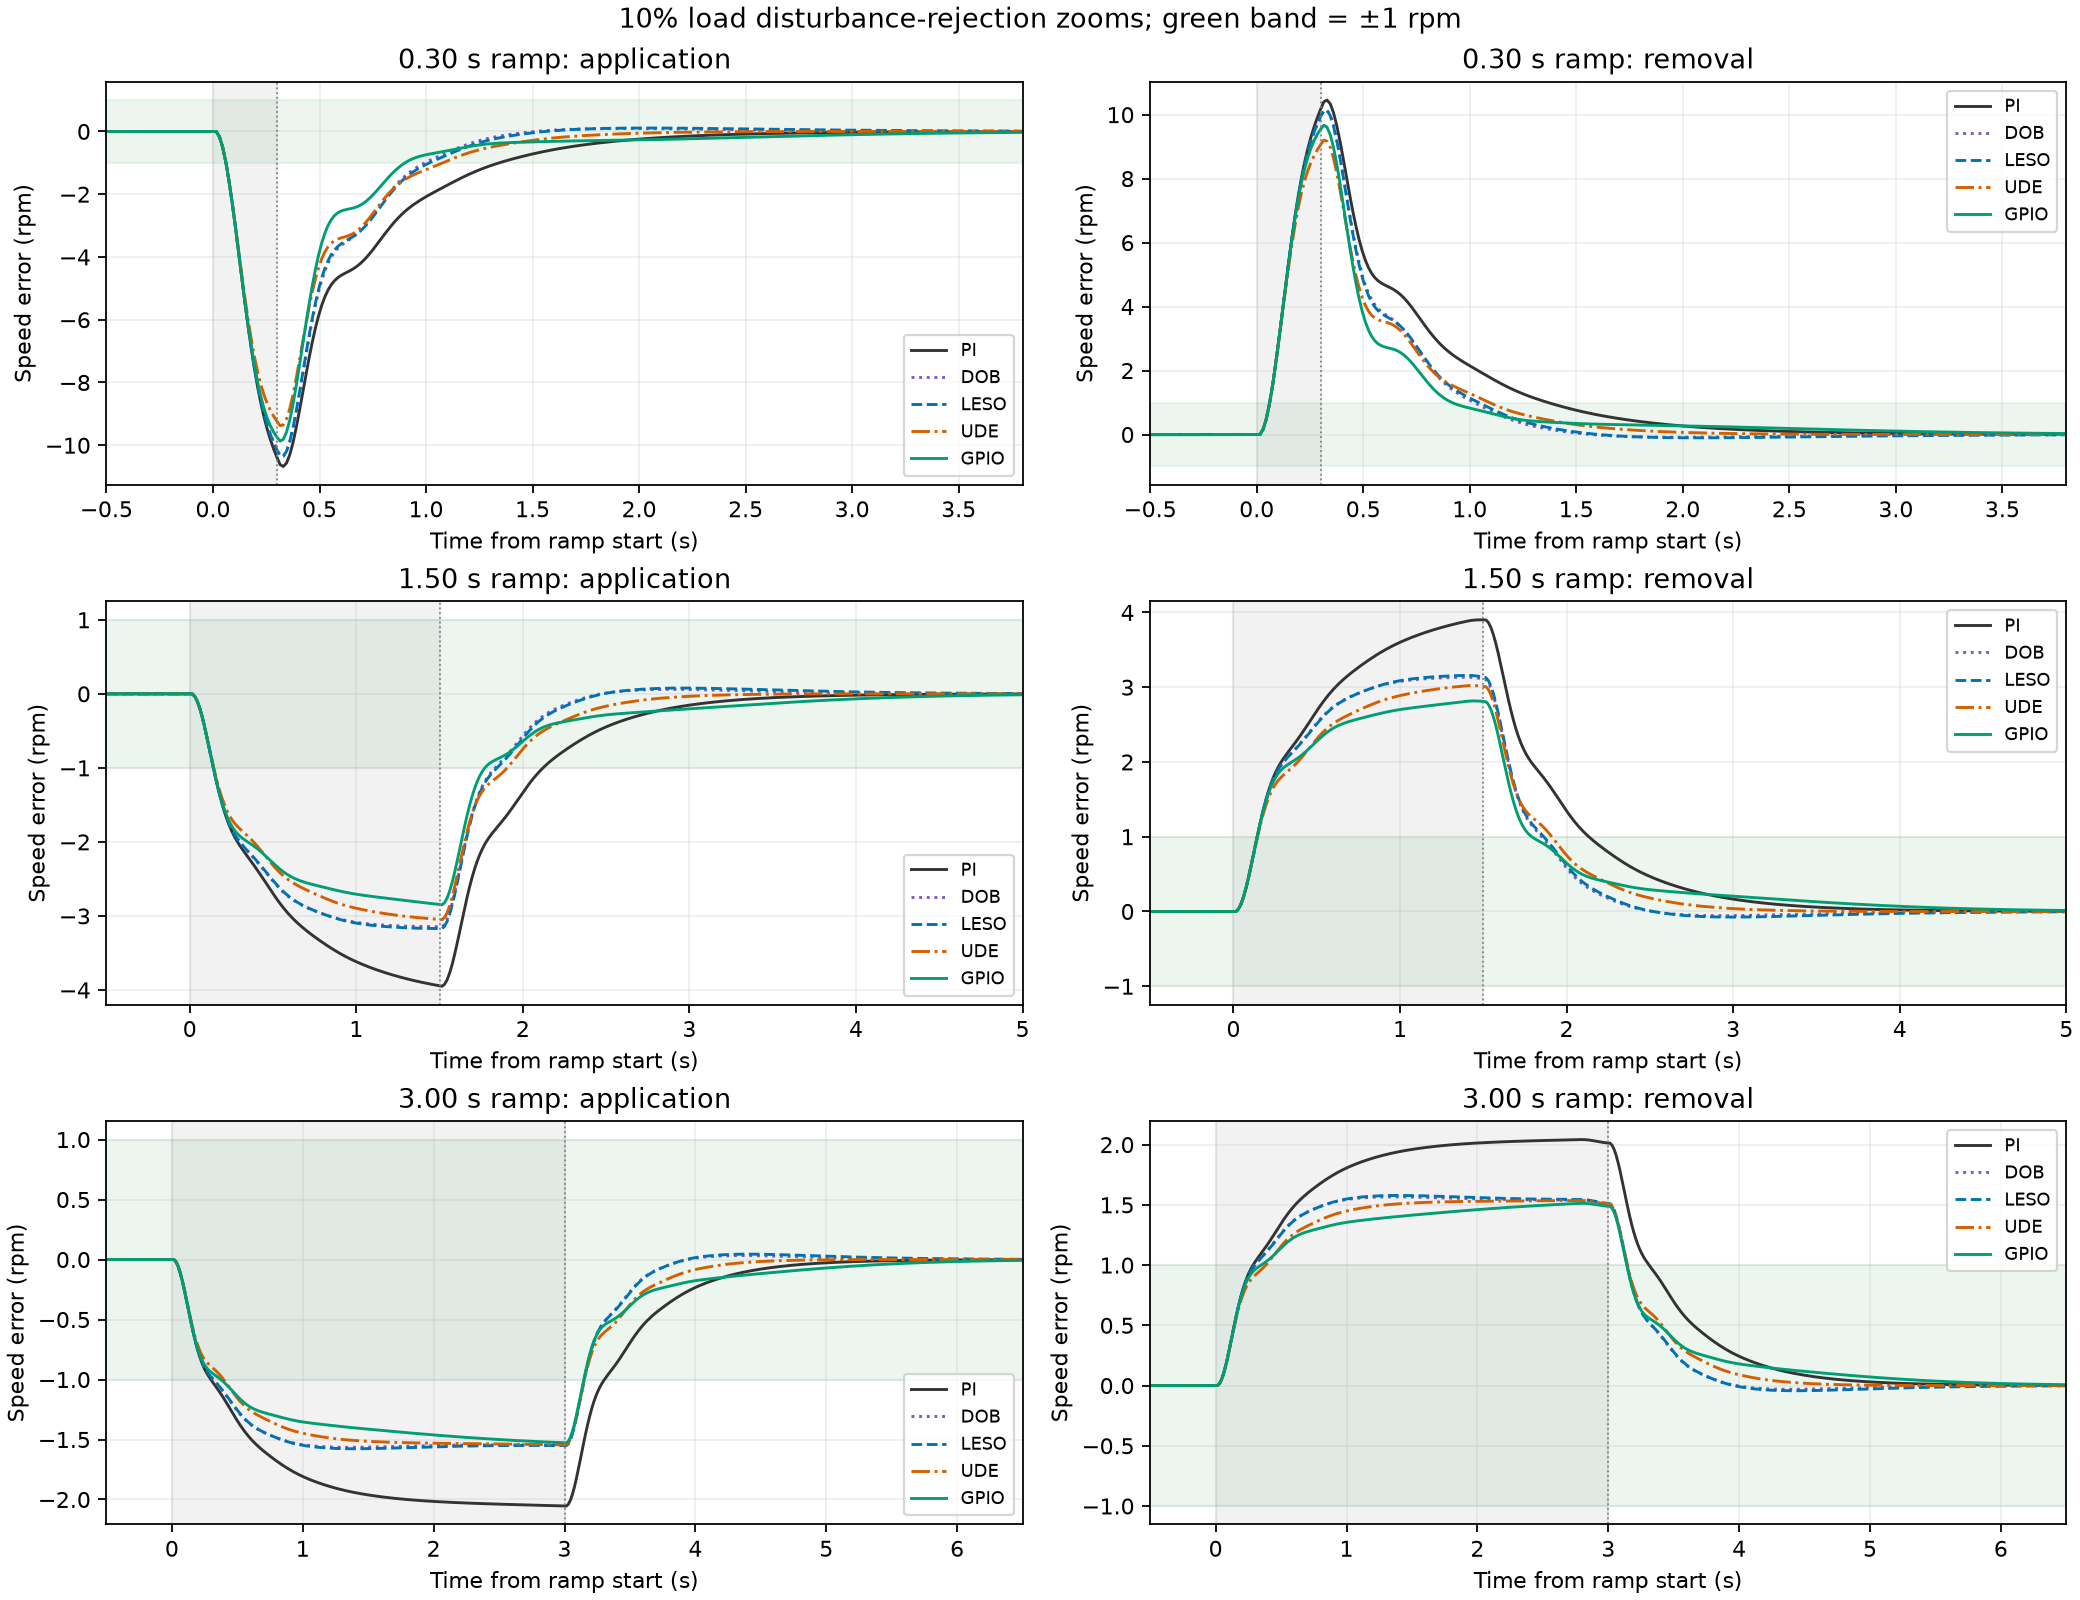
\includegraphics[width=.95\linewidth,height=.6\textheight,keepaspectratio]{early_literature_observers_9000rpm_10pct_20260912_211600_355_rejection_zooms.png}\caption{Zooms. Archived study figure.}\end{figure}

\subsection{Actuation and model validity}

{\scriptsize\setlength{\tabcolsep}{1.5mm}\begin{longtable}{>{\raggedright\arraybackslash}p{29.00mm}>{\raggedright\arraybackslash}p{29.00mm}>{\raggedright\arraybackslash}p{29.00mm}>{\raggedright\arraybackslash}p{29.00mm}>{\raggedright\arraybackslash}p{29.00mm}}\caption{LESO, UDE, and GPIO implementation and first comparison: Actuation and model validity. Archived values.}\\\toprule
Method & Fuel limit \% & Compensation clip \% & Fuel total variation lbm/s & Minimum compressor margin \%\\\midrule
\endfirsthead
Method & Fuel limit \% & Compensation clip \% & Fuel total variation lbm/s & Minimum compressor margin \%\\\midrule
\endhead
PI & 0.000 & 0.000 & 2.116 & 24.429\\
DOB & 0.000 & 0.000 & 2.136 & 24.322\\
LESO & 0.000 & 0.000 & 2.143 & 24.302\\
UDE & 0.000 & 0.000 & 2.144 & 24.389\\
GPIO & 0.000 & 0.000 & 2.174 & 24.161\\
\bottomrule\end{longtable}}

\subsection{Assessment}

\textbf{GPIO has the lowest RMSE in this fixed-setting test: 0.9509 rpm.} This is a measured result for the chosen nominal gain, observer poles and limits, not a universal ranking or optimally tuned benchmark. The existing DOB uses the fuller identified model; new observers use only its first fuel-to-acceleration coefficient as an approximate input gain.

\textbf{Practical recommendation:} start with UDE if implementation simplicity and peak rejection are the priorities; retain GPIO as the performance candidate when faster recovery justifies two extra observer states. LESO is a simpler-model substitute for the existing DOB here, but does not improve its overall RMSE. This recommendation is conditional on passing subsequent noise and robustness tests.

For the 0.30 s application ramp, post-ramp recovery is 1.050 s (PI), 0.705 s (DOB), 0.720 s (LESO), 0.780 s (UDE), and 0.615 s (GPIO). Thus UDE has the lowest peak, but is slower to enter the $\pm$1 rpm band than DOB and GPIO. For the 1.50 s ramp, GPIO application peak is 2.850 rpm versus 3.950 rpm for PI, with post-ramp recovery 0.285 versus 0.630 s. At 3.00 s, after-ramp recovery differs by only one sample or less among the augmented methods.

Relative to the existing DOB, UDE lowers RMSE by about 6.58\% and GPIO by 8.37\%. Neither fuel nor compensation saturation occurs. GPIO has the greatest fuel total variation (2.174 versus 2.116 lbm/s for PI) and the highest peak fuel (1.344 versus 1.333 lbm/s), illustrating a small actuation tradeoff. These total-variation values sum absolute sample-to-sample command changes; they are not fuel consumption.

UDE has the smallest state count and no raw derivative, but its direct speed term makes measurement-noise testing important. LESO is a simple general-purpose candidate. GPIO represents disturbance slope explicitly, at the cost of an additional state and stronger high-frequency correction. A shaft-power ramp is not necessarily a ramp in equivalent-fuel disturbance because the plant and sensor contribute to the residual.

Next compare separately tuned settings using an independent tuning case, then hold out load profiles for validation. Include sensor noise, delay variation, gain mismatch, fuel constraints and compressor margin. Do not choose a deployed method using speed RMSE alone: peak excursions, recovery, actuator variation and numerical/physical limits matter.

\subsection{Verification and reproduction}

All five actual Simulink trajectories contain 10001 samples through 150 s. Checks confirm identical shaft profiles, 9000 rpm evaluation demand, zero fuel disturbance and mechanical torque balance. The three new estimators are independently replayed from logged sensed speed and applied fuel with their exact discrete state equations. PI and existing DOB responses reproduce the preceding 10\% study. Detailed numerical errors are in verification.json.

Run \path|out=run_tmats_literature_comparison;| in MATLAB, then \path|summarize_literature_observers.py| in Python. The new model is \path|GasTurbine_Dyn_Template_GPT_DOB_PTO_ALT.mdl|; original models are preserved. Load the model first, then select an alternative with \path|tmats_literature_setup(2)| (LESO), \path|(3)| (UDE) or \path|(4)| (GPIO) before simulation; its PreLoadFcn initializes LESO by default. Observer pole stability does not establish nonlinear closed-loop robustness. No noisy or hardware experiment is claimed.


\section{Interpretation of the observer comparison} The accepted runs provide local evidence that these configured observers can reduce the recorded disturbance error. The rejected high-load cases restrict the scope of that evidence. Since load percentages are defined relative to operating-point turbine power, identical percentages at 9000 and 9500 rpm are not identical physical extraction powers. The tables compare controllers within a scenario; they do not estimate a universal observer ranking.
